%Version 3.1 December 2024
% See section 11 of the User Manual for version history
%
%%%%%%%%%%%%%%%%%%%%%%%%%%%%%%%%%%%%%%%%%%%%%%%%%%%%%%%%%%%%%%%%%%%%%%
%%                                                                 %%
%% Please do not use \input{...} to include other tex files.       %%
%% Submit your LaTeX manuscript as one .tex document.              %%
%%                                                                 %%
%% All additional figures and files should be attached             %%
%% separately and not embedded in the \TeX\ document itself.       %%
%%                                                                 %%
%%%%%%%%%%%%%%%%%%%%%%%%%%%%%%%%%%%%%%%%%%%%%%%%%%%%%%%%%%%%%%%%%%%%%

%%\documentclass[referee,sn-basic]{sn-jnl}% referee option is meant for double line spacing

%%=======================================================%%
%% to print line numbers in the margin use lineno option %%
%%=======================================================%%

%%\documentclass[lineno,pdflatex,sn-basic]{sn-jnl}% Basic Springer Nature Reference Style/Chemistry Reference Style

%%=========================================================================================%%
%% the documentclass is set to pdflatex as default. You can delete it if not appropriate.  %%
%%=========================================================================================%%

%%\documentclass[sn-basic]{sn-jnl}% Basic Springer Nature Reference Style/Chemistry Reference Style

%%Note: the following reference styles support Namedate and Numbered referencing. By default the style follows the most common style. To switch between the options you can add or remove �Numbered� in the optional parenthesis. 
%%The option is available for: sn-basic.bst, sn-chicago.bst%  
 
%%\documentclass[pdflatex,sn-nature]{sn-jnl}% Style for submissions to Nature Portfolio journals
%%\documentclass[pdflatex,sn-basic]{sn-jnl}% Basic Springer Nature Reference Style/Chemistry Reference Style
\documentclass[pdflatex,sn-mathphys-num,iicol]{sn-jnl}% Math and Physical Sciences Numbered Reference Style
%%\documentclass[pdflatex,sn-mathphys-ay]{sn-jnl}% Math and Physical Sciences Author Year Reference Style
%%\documentclass[pdflatex,sn-aps]{sn-jnl}% American Physical Society (APS) Reference Style
%%\documentclass[pdflatex,sn-vancouver-num]{sn-jnl}% Vancouver Numbered Reference Style
%%\documentclass[pdflatex,sn-vancouver-ay]{sn-jnl}% Vancouver Author Year Reference Style
%%\documentclass[pdflatex,sn-apa]{sn-jnl}% APA Reference Style
%%\documentclass[pdflatex,sn-chicago]{sn-jnl}% Chicago-based Humanities Reference Style

%%%% Standard Packages
%%<additional latex packages if required can be included here>

\usepackage{graphicx}%
\usepackage{multirow}%
\usepackage{amsmath,amssymb,amsfonts}%
\usepackage{amsthm}%
\usepackage{mathrsfs}%
\usepackage[title]{appendix}%
\usepackage{xcolor}%
\usepackage{textcomp}%
\usepackage{manyfoot}%
\usepackage{booktabs}%
\usepackage{algorithm}%
\usepackage{algorithmicx}%
\usepackage{algpseudocode}%
\usepackage{listings}%
\usepackage{subcaption}%
%\usepackage{multicol}
%\usepackage[margin=1.5cm]{geometry}
% Paper width: 21cm (A4)
% Desired left margin: 1.5cm
% Desired right margin: 1.5cm
% Therefore, textwidth = 21 - 1.5 - 1.5 = 18cm

%\setlength{\textwidth}{18cm}
%
%% For ODD pages (left margin = 1.5cm):
%% Left margin = 1in + \oddsidemargin => 2.54cm + \oddsidemargin = 1.5cm
%% => \oddsidemargin = 1.5 - 2.54 = -1.04cm
%\setlength{\oddsidemargin}{-1.04cm}
%
%% For EVEN pages (if twoside is active, right margin becomes the left margin on even pages):
%\setlength{\evensidemargin}{-1.04cm} % If you want 1.5cm margins on both sides for both pages.
%
%% Remove extra horizontal offset
%\setlength{\hoffset}{0pt}
% \headheight、\headsep、\footskip
%%%%

%%%%%=============================================================================%%%%
%%%%  Remarks: This template is provided to aid authors with the preparation
%%%%  of original research articles intended for submission to journals published 
%%%%  by Springer Nature. The guidance has been prepared in partnership with 
%%%%  production teams to conform to Springer Nature technical requirements. 
%%%%  Editorial and presentation requirements differ among journal portfolios and 
%%%%  research disciplines. You may find sections in this template are irrelevant 
%%%%  to your work and are empowered to omit any such section if allowed by the 
%%%%  journal you intend to submit to. The submission guidelines and policies 
%%%%  of the journal take precedence. A detailed User Manual is available in the 
%%%%  template package for technical guidance.
%%%%%=============================================================================%%%%

%% as per the requirement new theorem styles can be included as shown below
\theoremstyle{thmstyleone}%
\newtheorem{theorem}{Theorem}%  meant for continuous numbers
%%\newtheorem{theorem}{Theorem}[section]% meant for sectionwise numbers
%% optional argument [theorem] produces theorem numbering sequence instead of independent numbers for Proposition
\newtheorem{proposition}[theorem]{Proposition}% 
%%\newtheorem{proposition}{Proposition}% to get separate numbers for theorem and proposition etc.

\theoremstyle{thmstyletwo}%
\newtheorem{example}{Example}%
\newtheorem{remark}{Remark}%

\theoremstyle{thmstylethree}%
\newtheorem{definition}{Definition}%

\raggedbottom
%%\unnumbered% uncomment this for unnumbered level heads

\begin{document}

\title{Graph Representation Learning for Student Sectioning: A Node2Vec-Based Approach}

%%=============================================================%%
%% GivenName	-> \fnm{Joergen W.}
%% Particle	-> \spfx{van der} -> surname prefix
%% FamilyName	-> \sur{Ploeg}
%% Suffix	-> \sfx{IV}
%% \author*[1,2]{\fnm{Joergen W.} \spfx{van der} \sur{Ploeg} 
%%  \sfx{IV}}\email{iauthor@gmail.com}
%%=============================================================%%

\author*[1,2]{\fnm{Mahmood} \sur{Amintoosi}}\email{m.amintoosi@um.ac.ir}

\affil[1]{\orgdiv{Computer Science Division, Department of Applied Mathematics, Faculty of Mathematical Sciences}, \orgname{Ferdowsi University of Mashhad}, \orgaddress{
%\street{Street}, 
\city{P. O. Box 1159, Mashhad 91775}, %\postcode{100190}, \state{State}, 
\country{Iran}}}

\affil[2]{\orgdiv{Graph Theory and its Applications Lab.}, \orgname{Faculty of Mathematical Sciences, Ferdowsi University of Mashhad},  \orgaddress{
%\street{Street}, 
\city{Mashhad}, 
%\postcode{10587}, \state{State},
 \country{Iran}}
 %\orcid
 {ORCID: 0000-0001-9640-6475}
 }




%%==================================%%
%% Sample for unstructured abstract %%
%%==================================%%
\abstract{Student sectioning is a fundamental subproblem of university course timetabling that aims to partition students into sections while preserving scheduling flexibility and efficient resource utilization. Classical clustering-based approaches typically represent students using binary student--course enrollment matrices, which may not adequately capture the relational structure induced by shared course participation.

This paper revisits student sectioning from the perspective of graph representation learning, a powerful technique in artificial intelligence for learning low-dimensional representations from relational data. We construct a weighted student co-enrollment graph after removing constant features, and employ Node2Vec to learn low-dimensional student embeddings from biased random-walk contexts. The learned representations are then provided to standard clustering algorithms for section formation. To distinguish graph-based representation learning from dimensionality reduction and direct graph clustering, we compare the proposed approach with the conventional enrollment representation, PCA followed by KMeans, and spectral clustering on the co-enrollment graph.

Experiments on six real-world university courses comprising 341 student-course enrollments from an underlying dataset of 210 students demonstrate that Node2Vec achieves a 64\% relative improvement in clustering quality over the strongest baseline (PCA followed by KMeans) when using the optimal configuration identified through grid search ($p=2.0$, $q=1.0$, $d=1$). The proposed method consistently surpasses conventional representations across all evaluated courses (100\% win rate), providing strong evidence for practical significance. 
The results indicate that graph representation learning can capture useful structural information beyond conventional dimensionality reduction. Notably, the best performance is achieved with a single embedding dimension, suggesting that the co-enrollment graph structure provides sufficient discriminatory information for effective student sectioning. The proposed approach can be incorporated into existing student sectioning pipelines without modifying the downstream clustering algorithms, providing a simple framework for improving student groupings used in subsequent timetabling processes.
}

\keywords{Student sectioning, Graph representation learning, Node2Vec, DeepWalk, Course timetabling, Clustering}
%%\pacs[JEL Classification]{D8, H51}



%%\pacs[MSC Classification]{35A01, 65L10, 65L12, 65L20, 65L70}
\maketitle

\clearpage

%% Use \section commands to start the section
\section{Introduction}

Student sectioning is a classical subproblem of university course timetabling, aiming to divide enrolled students into balanced instructional sections while preserving the flexibility required for subsequent scheduling and resource allocation. The quality of sectioning can affect downstream timetabling by influencing the compatibility of student groups with available classrooms, instructors, and time slots. Consequently, student sectioning has long been studied as an important problem within educational scheduling and constraint satisfaction.

Research on student sectioning dates back more than two decades. Early studies investigated clustering-based approaches, including fuzzy clustering with feature selection and later nature-inspired optimization methods, demonstrating the potential of data-driven grouping strategies for student sectioning \cite{Amintoosi2004Fuzzy,Amintoosi2005Feature,Amintoosi2007FishSchool}. Other studies formulated student sectioning as an optimization or constraint programming problem within larger university timetabling systems \cite{aubin1989large,hertz1998constructing,Carter2001Comprehensive,Alvarez-Valdes2000,Muller2010}. Together, these studies established important computational foundations for student sectioning and highlighted its role in educational resource management.

A common representation in clustering-based approaches is a student--course enrollment matrix, in which each student is represented by a binary vector indicating the courses in which the student is enrolled. This representation provides a direct description of student--course relationships and can be effective for sectioning. However, students can also be viewed as nodes in a relational network, where students are connected according to shared course enrollments. Such a representation makes it possible to model relationships between students not only through individual shared courses, but also through their connectivity patterns in the resulting co-enrollment network.

An important question is therefore whether the relational structure of student enrollments can provide useful information beyond the original enrollment representation. This question is particularly relevant because conventional dimensionality-reduction techniques can already substantially improve clustering in high-dimensional enrollment spaces. Thus, evaluating graph-based representations requires distinguishing their contribution from the general benefit of reducing the dimensionality of the input space.

Graph representation learning provides a natural framework for addressing this question. In particular, random-walk-based methods such as Node2Vec learn continuous node representations from the contexts generated by biased random walks on a graph \cite{perozzi2014deepwalk,node2vec_grover2016}. Node2Vec extends DeepWalk by introducing return and in-out parameters that control the balance between local and global graph exploration. These representations can encode structural relationships among nodes and provide low-dimensional features that can subsequently be used by conventional machine-learning algorithms.

Graph representation learning appears to have received limited attention in the student sectioning literature, despite the natural relational structure of student co-enrollment data. This motivates the central question addressed in this paper:

\begin{quotation}
Can graph representation learning provide student representations that improve sectioning quality beyond both conventional enrollment representations and standard dimensionality reduction?
\end{quotation}

To investigate this question, we model student enrollments as a weighted co-enrollment graph and learn student embeddings using Node2Vec~\cite{node2vec_grover2016}, a random-walk-based graph representation learning method that extends DeepWalk~\cite{perozzi2014deepwalk} through biased random walks controlled by return and in-out parameters. The learned embeddings are then supplied to standard clustering algorithms for section formation. Importantly, the clustering stage is kept unchanged, allowing the effect of the learned representation to be examined independently of the choice of clustering algorithm. To assess whether the observed improvement is attributable merely to dimensionality reduction, we compare the proposed representation with a PCA-based representation having the same dimensionality. We also include spectral clustering as a graph-based baseline.

Experimental results on six real-world university courses comprising 341 student-course enrollments from 210 students show that Node2Vec provides substantially better clustering quality than the conventional enrollment representation and spectral clustering. PCA also produces a considerable improvement, but Node2Vec achieves higher average Silhouette Scores than PCA followed by KMeans, indicating that graph-based representations capture useful structural information beyond linear dimensionality reduction. Additional experiments investigate parameter sensitivity, clustering stability, computational cost, and the resulting low-dimensional representations.

The main contributions of this paper are summarized as follows.

\begin{enumerate}

\item We investigate the application of graph representation learning to the student sectioning problem by constructing a weighted student co-enrollment graph and learning student representations using Node2Vec, a random-walk-based method with controllable exploration bias. While Node2Vec is an established technique in network analysis, its application to student sectioning via weighted co-enrollment graphs has received limited attention, and we demonstrate substantial improvements over conventional approaches.

\item We provide a crucial ablation-like analysis by systematically comparing graph-based representations with both the conventional student--course enrollment representation and a PCA-based dimensionality-reduction baseline. This analysis separates the effect of generic dimensionality reduction (PCA) from actual structural graph learning (Node2Vec), proving that the structural information captured by random walks provides additional value beyond just compressing data. Spectral clustering is additionally evaluated as a direct graph-based clustering baseline.

\item We empirically demonstrate on six real-world university courses that Node2Vec consistently outperforms both the conventional representation and PCA-based dimensionality reduction across all evaluated courses. Due to the limited number of course-specific sectioning instances ($n=6$) available from a single institutional dataset, we focus on effect sizes and consistency of improvement rather than formal statistical hypothesis testing, providing strong evidence for practical significance.

\item We provide comprehensive empirical analyses of Node2Vec parameter sensitivity, clustering stability across 20 random seeds, practical significance through effect sizes and consistency, runtime, and embedding structure, providing a detailed characterization of the proposed framework.

\item We show that graph-based student representations can be seamlessly incorporated into existing clustering-based sectioning pipelines without modifying the downstream clustering algorithms, providing a simple and practical framework for improving student groupings used in subsequent timetabling processes.

\end{enumerate}

The remainder of this paper is organized as follows. Section~\ref{sec:related} reviews previous work on student sectioning and graph representation learning. Section~\ref{sec:methods} presents the proposed framework. Section~\ref{sec:experiments} reports the experimental results and comparative analyses. Section~\ref{sec:discussion} discusses the findings, while Section~\ref{sec:conclusion} concludes the paper.

\section{Related Work}
\label{sec:related}

This work revisits the classical student sectioning problem from the perspective of graph representation learning. The related literature is therefore reviewed from two complementary directions: classical approaches to student sectioning and course timetabling, and graph representation learning for relational data. We then position the present study at the intersection of these two directions.

\subsection{Student Sectioning and Course Timetabling}

Student sectioning is a fundamental component of university course timetabling and educational scheduling. Its objective is to partition students into instructional sections while satisfying scheduling constraints and making efficient use of institutional resources. Because section assignments affect the flexibility of subsequent timetable construction, student sectioning has long been studied as an optimization problem within operations research and constraint programming.

Early studies primarily formulated student sectioning as part of larger timetabling systems. Aubin and Ferland \cite{aubin1989large} incorporated section generation into a university timetabling framework, while Hertz and Robert \cite{hertz1998constructing} decomposed the scheduling process into assignment subproblems including student sectioning. Carter \cite{Carter2001Comprehensive} considered grouping students according to course selections before timetable construction with the objective of reducing subsequent scheduling conflicts. Other approaches employed tabu search \cite{Alvarez-Valdes2000} and priority-based constraint satisfaction techniques \cite{feldman1990optimization}. These studies established student sectioning as an important component of integrated university timetabling systems.

Data-driven approaches subsequently introduced clustering techniques for student sectioning. Fuzzy clustering with feature selection was proposed in \cite{Amintoosi2004Fuzzy,Amintoosi2005Feature}, representing students through enrollment-based feature vectors and applying fuzzy c-means clustering together with criteria for evaluating section balance. A Fish School clustering algorithm was later developed specifically for student sectioning, demonstrating the applicability of nature-inspired optimization to this problem \cite{Amintoosi2007FishSchool}. Although these approaches differ in their optimization mechanisms, they generally represent students through their course enrollment information and subsequently apply a clustering or partitioning procedure.

\subsection{Graph Representation Learning}

Graph representation learning provides an alternative way of representing objects when their relationships are an important source of information. Instead of treating observations as independent feature vectors, graph embedding methods exploit graph topology to learn continuous low-dimensional representations that reflect structural relationships among nodes.

DeepWalk \cite{perozzi2014deepwalk} introduced a widely adopted random-walk-based approach to graph representation learning by generating truncated random walks and applying the Skip-Gram model to the resulting node sequences. The learned embeddings capture patterns of node co-occurrence induced by the graph structure. Node2Vec \cite{node2vec_grover2016} subsequently extended this framework through biased random walks that provide greater control over local and global graph exploration. Related studies have investigated weighted random walks and other graph sampling strategies \cite{Qi2024Weighted}. Graph representation and graph-based learning techniques have also been employed in a variety of application-oriented problems, including network embedding, structured optimization, and graph neural network-based anomaly detection \cite{AlJreidy2024Clustering,Solgi2022GraphPrototypical,Luo2022LinkPrediction}.

These developments illustrate the broader applicability of graph-based learning beyond conventional graph benchmarks. In particular, they suggest that exploiting relational structure can be useful when the relationships among entities contain information that is difficult to capture directly from their original feature descriptions.

\subsection{Graph Representation Learning for Student Sectioning}

The student--course enrollment data used in sectioning naturally induces a relational structure among students. Two students can be connected according to the courses they jointly attend, resulting in a student co-enrollment graph. Such a graph provides an alternative representation of the same underlying enrollment information and makes it possible to investigate whether structural patterns in the co-enrollment network can improve student grouping.

To our knowledge, the use of graph representation learning as an explicit representation stage for student sectioning has received little attention. The present work investigates this intersection by constructing a weighted student co-enrollment graph and learning student embeddings using Node2Vec. The resulting embeddings are subsequently supplied to standard clustering algorithms, without modifying the clustering procedure itself.

An important aspect of the present study is that the improvement is not evaluated only against the original high-dimensional enrollment representation. Since dimensionality reduction can itself substantially affect clustering performance, we additionally consider PCA followed by KMeans as a representation-based baseline with the same embedding dimensionality as Node2Vec. We also evaluate spectral clustering directly on the co-enrollment graph as a graph-based clustering baseline. These comparisons allow us to examine whether the observed benefit of Node2Vec is attributable merely to dimensionality reduction or whether graph-based representation learning provides additional useful information for student sectioning.

The present study therefore complements earlier clustering-based approaches to student sectioning rather than replacing them. Its central objective is to examine whether a Node2Vec-based representation learning stage can improve the quality of student representations while leaving the subsequent clustering pipeline unchanged.

\section{Methodology}
\label{sec:methods}

The proposed framework revisits the student sectioning problem from a graph representation learning perspective. Instead of representing students solely through a binary student--course enrollment matrix, we construct a student co-enrollment graph and learn continuous vector representations of students from the topology of this graph. These representations are subsequently used as input to conventional clustering algorithms to generate student sections.

The overall framework consists of four main stages: (1) construction of the student co-enrollment graph, (2) graph representation learning using random walks, (3) clustering of the learned student representations, and (4) evaluation of the resulting student sections. Figure~\ref{fig:framework} illustrates the overall workflow.

\begin{figure}[t]
\centering
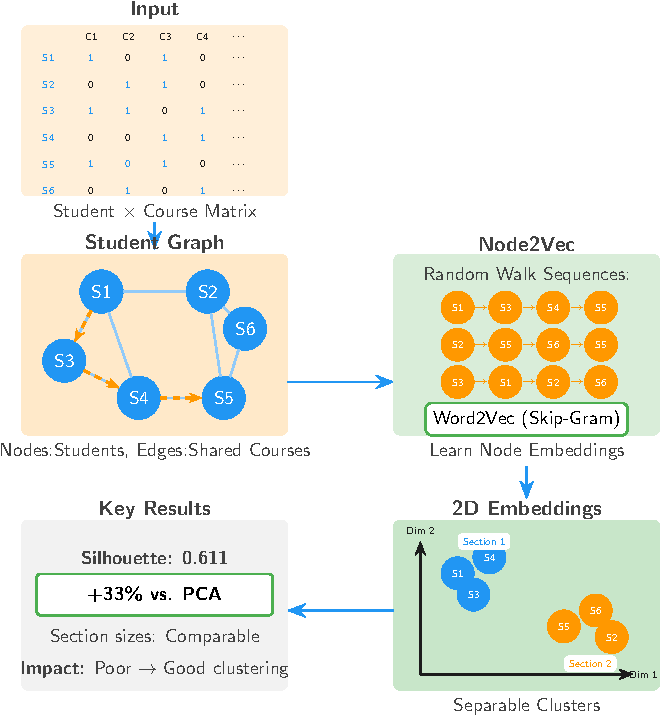
\includegraphics[width=1\linewidth]{graphical_abstract.pdf}
\caption{Overview of the proposed framework. A student--course enrollment matrix is transformed into a student co-enrollment graph, from which random walks are generated and fed to a Skip-Gram (Word2Vec) model to learn low-dimensional student embeddings. The learned embeddings are then clustered to produce student sections.}
\label{fig:framework}
\end{figure}

\subsection{Student Co-enrollment Graph}
\label{subsec:graph_construction}

Let $S=\{s_1,s_2,\ldots,s_n\}$ denote the set of students and let $C=\{c_1,c_2,\ldots,c_m\}$ denote the set of courses. Student enrollment information can be represented by a binary matrix $X\in\{0,1\}^{n\times m}$, where

$$
X_{ic} =
\begin{cases}
1, & \text{if student } s_i \text{ is enrolled in course } c,\\
0, & \text{otherwise}.
\end{cases}
$$

Although the enrollment matrix provides a direct representation of student--course relationships, it does not explicitly represent relationships between students. We therefore transform the enrollment information into a student co-enrollment graph.

We define an undirected weighted graph $G=(V,E,W)$, where each vertex $v_i\in V$ corresponds to a student $s_i$. An edge $(v_i,v_j)\in E$ is established when students $s_i$ and $s_j$ share at least one enrolled course. The edge weight measures the strength of their co-enrollment relationship.

In the basic version of the proposed framework, the edge weight between students $s_i$ and $s_j$ is defined as the number of courses in which they are simultaneously enrolled:

$$
w_{ij}=\sum_{c\in C}X_{ic}X_{jc}.
$$

Consequently, students who share several courses are connected by stronger edges, whereas students who share only one course have a weaker connection. This weighted representation preserves more information than a binary adjacency matrix and provides a natural basis for subsequent random-walk-based representation learning.

The resulting graph can be represented by a weighted adjacency matrix $W\in\mathbb{R}^{n\times n}$, where $W_{ij}=w_{ij}$ for connected students and $W_{ij}=0$ otherwise. Because the co-enrollment relationship is symmetric, the resulting graph is undirected and $W_{ij}=W_{ji}$.

\subsection{Preprocessing: Removal of Constant Features}
\label{subsec:preprocessing}

Before constructing any representation, we apply a standard preprocessing step to the student--course enrollment matrix. Courses that are taken by every student in a sectioning instance have zero variance and provide no discriminative information for clustering. Such constant features are therefore removed from the enrollment matrix before any representation or graph is constructed.

Specifically, for each target course, we identify courses $c$ for which $X_{ic}=1$ for all students $s_i$ in the student set. These universally shared courses are removed, and the remaining enrollment matrix is used for all subsequent steps: BoW representation, PCA projection, graph construction, and random-walk-based embedding. This ensures that all methods operate on the same preprocessed data.

In the six sectioning instances studied here, exactly one constant course is identified and removed per instance. The resulting graphs are non-complete, with average density approximately $0.72$, in contrast to the fully connected graphs that arise when the constant course is included.

\subsection{Random-walk-based Student Representation Learning}
\label{subsec:embedding}

After constructing the co-enrollment graph, we learn a vector representation for each student using Node2Vec \cite{node2vec_grover2016}, a random-walk-based graph embedding method. The main idea is to treat the graph analogously to a corpus: students correspond to words, and random walks correspond to sentences. Students that frequently occur in similar graph contexts are therefore expected to obtain similar vector representations.

Node2Vec generates biased random walks in which the transition probability depends on both the previous and the next-to-previous node in the walk. Let $u$ denote the previous node and $v$ denote the current node. The unnormalized transition probability to a neighbor $x$ is defined as

$$
\pi(v,x) = \alpha_{pq}(u,x) \cdot w_{vx},
$$

where $w_{vx}$ is the edge weight and the bias factor $\alpha_{pq}(u,x)$ is

$$
\alpha_{pq}(u,x) =
\begin{cases}
1/p, & \text{if } d(u,x)=0,\\
1, & \text{if } d(u,x)=1,\\
1/q, & \text{if } d(u,x)=2,
\end{cases}
$$

where $d(u,x)$ denotes the shortest-path distance between nodes $u$ and $x$. The parameter $p$ controls the likelihood of returning to the previous node (return parameter), and $q$ controls whether the walk explores locally (BFS-like, $q<1$) or globally (DFS-like, $q>1$). Setting $p=1$ and $q=1$ recovers the standard unbiased random walk used by DeepWalk.

Thus, students with stronger co-enrollment relationships have a higher probability of being visited during the random walk, and the bias parameters allow the walk to emphasize either local neighborhood structure or broader graph exploration. Repeating this procedure produces a collection of student sequences (Algorithm~\ref{alg:random_walk}),

$$
\mathcal{W}=\{W_1,W_2,\ldots,W_R\},
$$

where $R$ denotes the total number of generated walks.

The resulting walks capture both local and higher-order relationships in the student graph (Figure~\ref{fig:random-walk} illustrates an example walk). For example, two students who do not directly share a course may nevertheless occur frequently in similar random-walk contexts because they are connected through common groups of students. Such relationships cannot be directly captured by treating each student's enrollment vector independently.

\begin{figure}[t]
\centering
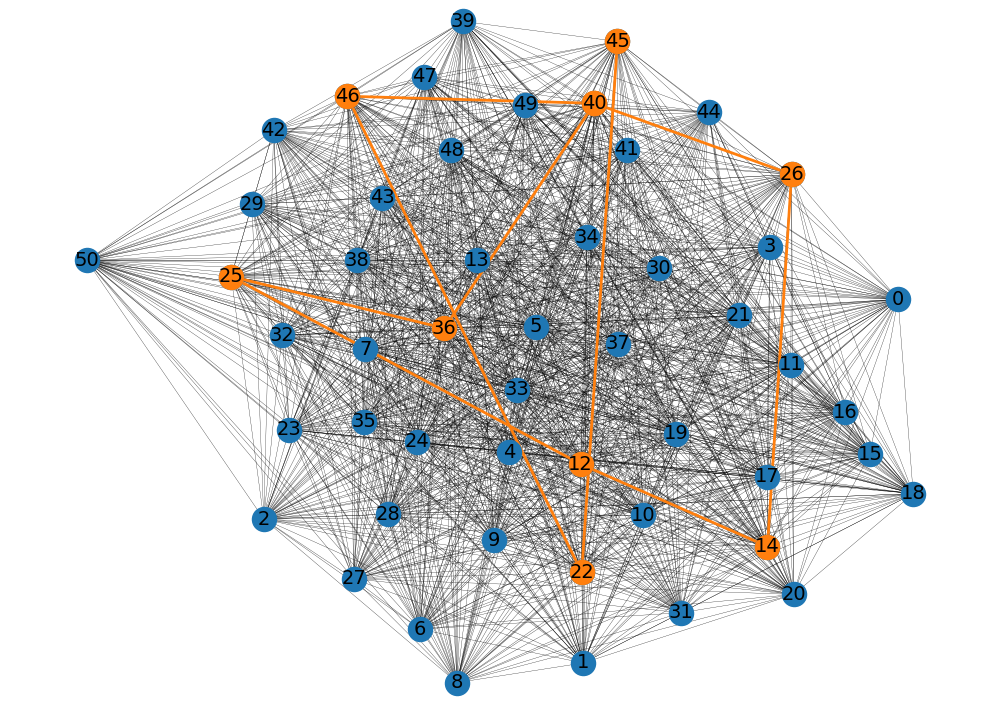
\includegraphics[width=1\linewidth]{random-walk-2-node40.png}
\caption{Example random walk on the student graph for Course~2, starting at node~40 and ending at node~45: $\{40, 36, 25, 12, 14, 26, 40, 46, 22, 45\}$. Students who share courses are connected, and the walk explores the local neighborhood structure.}
\label{fig:random-walk}
\end{figure}

\subsection{Learning Student Embeddings}
\label{subsec:deepwalk}

The generated random walks are used to learn low-dimensional student representations using a skip-gram objective. Let $z_v\in\mathbb{R}^d$ denote the embedding of student $v$, where $d$ is the embedding dimension. For a student $v$, the objective encourages students appearing within a context window of $v$ to have similar representations. Figure~\ref{fig:cbow_skipgram} illustrates the CBOW and Skip-gram architectures used in this learning stage.

\begin{figure}[t]
\centering
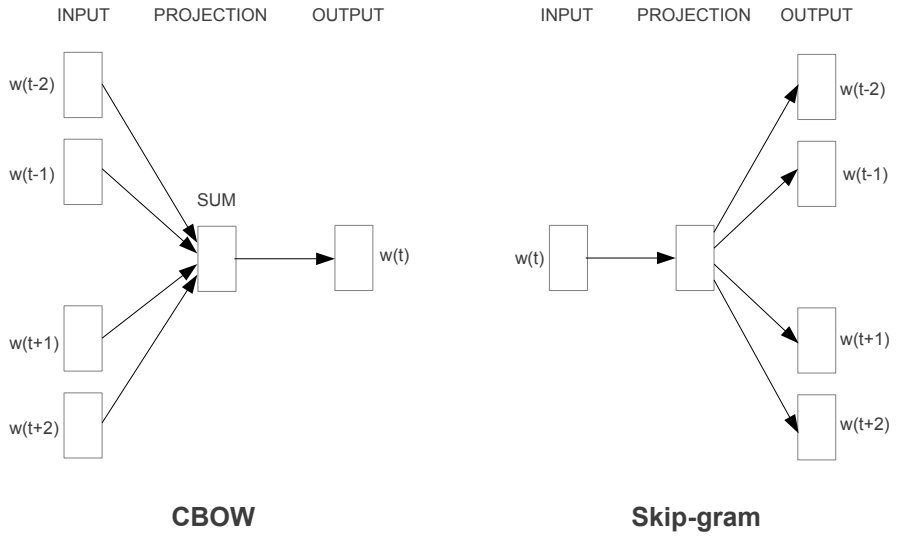
\includegraphics[width=1\linewidth]{CBOW-Skip-gram.png}
\caption{The CBOW architecture predicts the current word based on the context, and the Skip-gram predicts surrounding words given the current word~\cite{mikolov2013efficient}. In Node2Vec, nodes play the role of words and random-walk sequences play the role of sentences.}
\label{fig:cbow_skipgram}
\end{figure}

Given a context window of size $r$, the optimization objective can be expressed as

$$
\max_{\{z_v\}}
\sum_{v\in V}
\sum_{u\in C(v)}
\log P(u\mid v),
$$

where $C(v)$ denotes the set of students occurring within the specified context window of $v$ in the generated random walks.

The conditional probability can be modeled using the softmax function:

$$
P(u\mid v)
=
\frac{\exp(z_u^\top z_v)}
{\sum_{x\in V}\exp(z_x^\top z_v)}.
$$

In practice, negative sampling can be used to make the optimization computationally efficient. The resulting embedding matrix

$$
Z=
\begin{bmatrix}
z_1^\top\\
z_2^\top\\
\vdots\\
z_n^\top
\end{bmatrix}
\in\mathbb{R}^{n\times d}
$$

provides a continuous representation of all students.

The important distinction from the original enrollment representation is that each vector $z_i$ is learned from the structural context of student $s_i$ in the entire co-enrollment network. Consequently, the representation can capture indirect and higher-order similarities between students.



\begin{algorithm}[t]
\begin{algorithmic}[1]
\Require graph $G(V,E,W)$ constructed from student-course matrix, where students are its nodes. The input parameters are:\newline
return parameter $p$\newline
in-out parameter $q$\newline
walk length $L$\newline
number of walks per node $\gamma$\newline
embedding size $d$\newline
window size $w$\newline 
epochs $\epsilon$
\Ensure matrix of vertex (student) representations $\Phi \in \mathbb{R}^{|V| \times d}$
    \State $\mathcal{W} \gets$ GenerateRandomWalks($G, L, \gamma, p, q$) \Comment{Algorithm~\ref{alg:random_walk}}
    \State $\Phi \gets$  TrainWord2Vec($\mathcal{W}, d, w, \epsilon$) \Comment{Sect.~\ref{subsec:deepwalk}}
    \State \Return $\Phi$ 
\end{algorithmic}
\caption{Student Representation Learning using Node2Vec}
\label{alg:student-representation}
\end{algorithm}
Algorithm~\ref{alg:student-representation} summarizes the overall procedure: biased random walks are generated from the co-enrollment graph (line~1), and the Skip-Gram model is trained on these walks to produce the student embedding matrix $\Phi$ (line~2 of algorithm \ref{alg:student-representation}).

\subsection{Student Sectioning by Clustering}
\label{subsec:clustering}

Once the student embeddings have been learned, student sectioning is formulated as a clustering problem. Let $k$ denote the desired number of sections. A clustering algorithm partitions the set of student embeddings

$$
Z=\{z_1,z_2,\ldots,z_n\}
$$

into $k$ clusters,

$$
\mathcal{S}=\{S_1,S_2,\ldots,S_k\},
$$

where each cluster $S_j$ corresponds to a student section.

The proposed framework is deliberately independent of a particular clustering algorithm. This allows us to investigate whether the improvement comes from the learned graph representations rather than from a specific clustering technique. In our experiments, we therefore evaluate several widely used clustering methods, including K-means, affinity propagation, Gaussian mixture models, and hierarchical clustering.




For K-means, for example, the clustering objective is

$$
\min_{\{S_j\}_{j=1}^{k}}
\sum_{j=1}^{k}
\sum_{z_i\in S_j}
\left\|z_i-\mu_j\right\|_2^2,
$$

where $\mu_j$ denotes the centroid of section $S_j$.

The resulting clusters define the student sections used in the subsequent evaluation. A simple section balance metric $B = \min(|S_1|,|S_2|) / \max(|S_1|,|S_2|)$ for two sections (or the analogous ratio for $k>2$) can further characterize the practical suitability of the resulting sections, although a comprehensive evaluation of sectioning quality in the context of downstream timetabling constraints is beyond the scope of the present study.


\subsection{Baseline Representation}
\label{subsec:baseline}

To determine whether graph representation learning provides an advantage over conventional student representations, we establish a baseline based directly on the student--course enrollment matrix.

For each student $s_i$, the corresponding row of the enrollment matrix,

$$
x_i=(X_{i1},X_{i2},\ldots,X_{im}),
$$

is used as the student representation. Thus, students are represented directly by their binary course enrollment patterns without constructing a graph or learning an embedding.

The same clustering algorithms are then applied to these enrollment vectors. This provides a controlled comparison because the clustering stage remains unchanged and the principal difference between the two approaches is the representation used to describe students.

%\clearpage

Accordingly, the comparison considers two alternative pipelines:

{Enrollment representation}
$\rightarrow$ {Clustering},
and

{Graph representation}
$\rightarrow$
{Embedding}
$\rightarrow$
{Clustering}.

This design allows the contribution of graph representation learning to be evaluated independently of the choice of clustering algorithm.

\subsection{Hyperparameter Configuration}
\label{subsec:hyperparameters}

The graph embedding procedure contains several hyperparameters that may affect the quality of the learned representations. The principal parameters considered in this study include the embedding dimension $d$, the random-walk length $L$, the number of walks generated per student $\gamma$, and the context-window size $w$.

The embedding dimension controls the dimensionality of the learned student representations. A larger value provides greater representational capacity but may also increase computational cost and the risk of overfitting. The walk length determines how far the random walks explore the co-enrollment network, while the number of walks controls the amount of structural context available during training. The context-window size determines the range of neighboring positions considered when learning the embedding.

Rather than relying on a single arbitrary configuration, we conduct a comprehensive grid search over the Node2Vec-specific parameters $p$, $q$, and $d$ (Section~\ref{sec:grid_search}), as well as sensitivity experiments over the remaining hyperparameters. The purpose is not to optimize the method specifically for a particular dataset, but to examine whether the observed improvement is robust across reasonable parameter settings.

\subsection{Node2Vec Grid Search}
\label{sec:grid_search}

To identify the optimal Node2Vec configuration for student sectioning, we conduct a comprehensive grid search over the key hyperparameters that control the random-walk behavior and embedding dimensionality. Specifically, we evaluate all combinations of:

\begin{itemize}
\item Return parameter $p \in \{0.5, 1.0, 2.0\}$
\item In-out parameter $q \in \{0.5, 1.0, 2.0\}$
\item Embedding dimension $d \in \{1, 2, 3, 5, 10\}$
\end{itemize}

This yields $3 \times 3 \times 5 = 45$ unique configurations. Each configuration is evaluated on all six courses with a fixed random seed (seed = 42) to ensure reproducibility. For each course and configuration, we generate Node2Vec embeddings using $L=10$ walk length, $\gamma=80$ walks per node, window size $w=5$, and $\epsilon=30$ training epochs, followed by KMeans clustering with $k=2$ clusters. The primary evaluation metric is the average Silhouette Score across all six courses.

The grid search results are summarized in Figure~\ref{fig:grid_search_heatmaps}, which shows heatmaps of the average Silhouette Score for each $(p, q)$ combination at each embedding dimension $d$. Each heatmap uses an independent color scale to facilitate visual comparison of the variation within each dimension.

\begin{figure}[t]
\centering
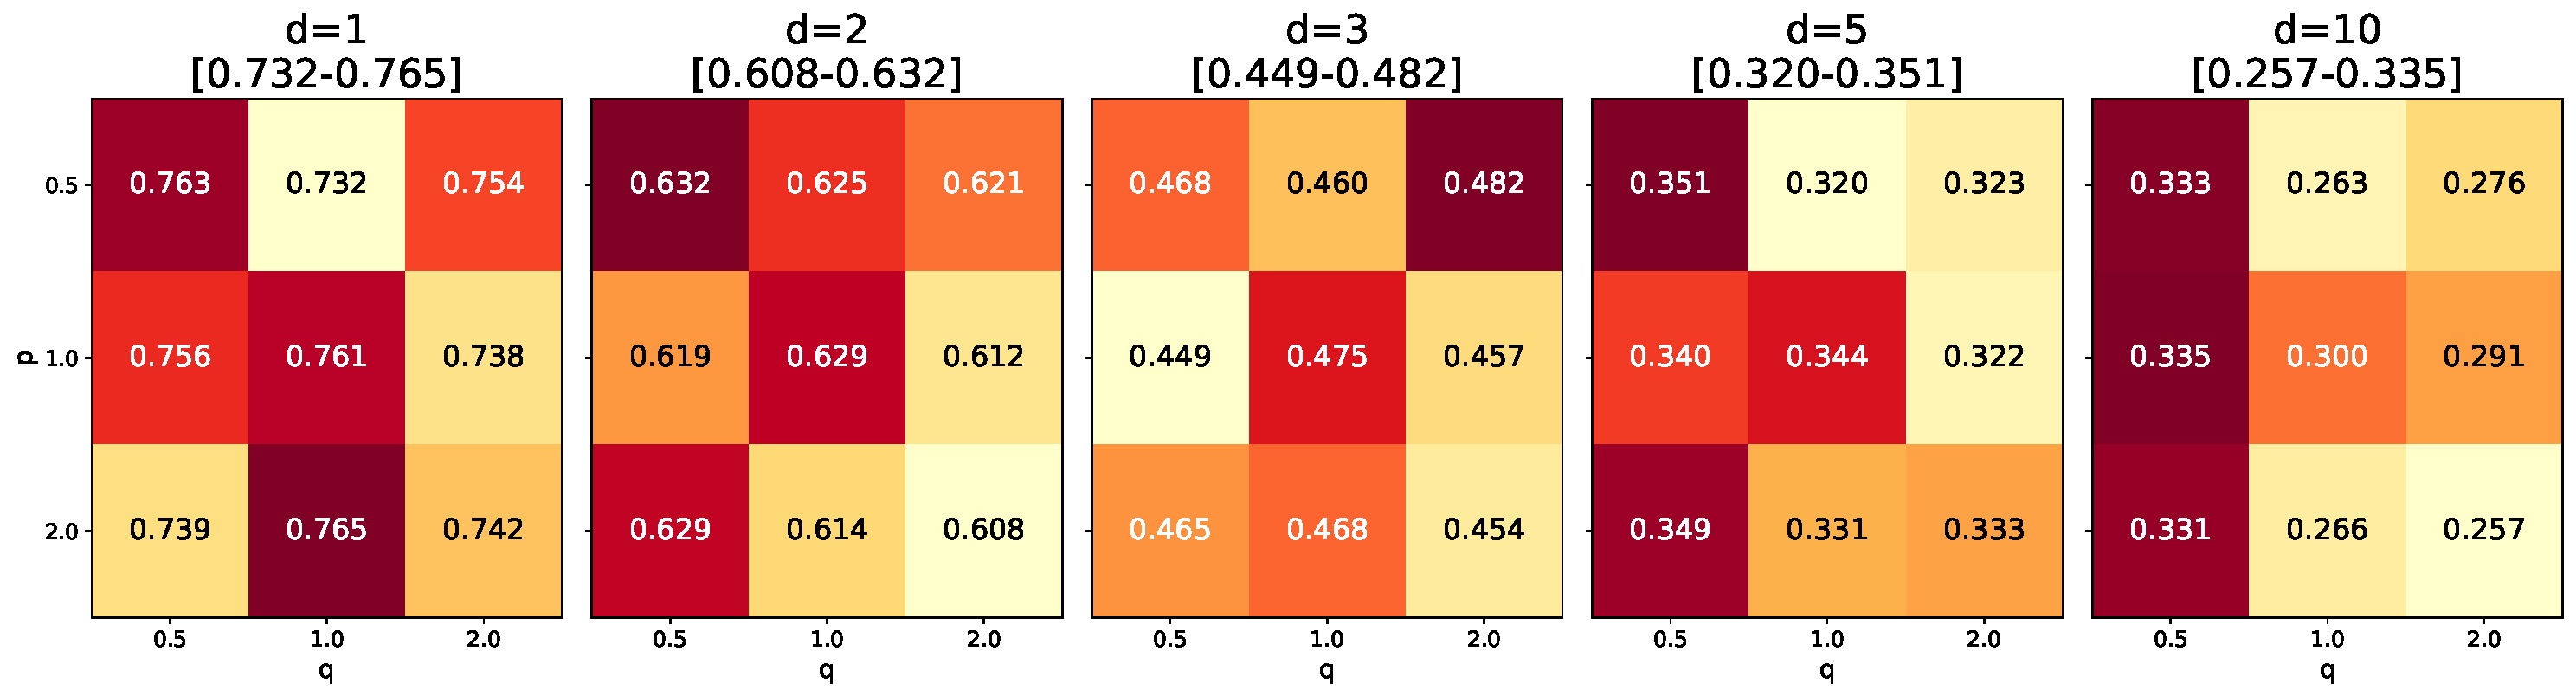
\includegraphics[width=1\linewidth]{grid_heatmap_all_d_independent.pdf}
\caption{Heatmaps of average Silhouette Score for the Node2Vec $(p, q, d)$ grid search. Each panel shows the mean Silhouette Score across six courses for a fixed embedding dimension $d$, with rows corresponding to the return parameter $p$ and columns to the in-out parameter $q$. Each panel uses an independent color normalization to highlight the variation within each dimension. The best overall configuration ($p=2.0$, $q=1.0$, $d=1$, avg. Silhouette = 0.765) is highlighted in the top-left panel.}
\label{fig:grid_search_heatmaps}
\end{figure}

The grid search reveals several important findings:

\begin{enumerate}
\item \textbf{Embedding dimension critically affects performance.} The best results are consistently achieved at $d=1$, with average Silhouette Scores ranging from $0.732$ to $0.765$. Performance degrades substantially as $d$ increases beyond 2, with $d=10$ yielding average Silhouette Scores below $0.4$ for most configurations. This suggests that the co-enrollment graph structure provides sufficient discriminatory information for student sectioning in a very low-dimensional space.

\item \textbf{The return parameter $p$ interacts with embedding dimension.} At $d=1$, higher values of $p$ (reducing the likelihood of returning to the previous node) tend to produce better clustering. The best configuration overall is $p=2.0$, $q=1.0$, $d=1$ with an average Silhouette Score of $0.765$. At higher dimensions, the effect of $p$ is less pronounced.

\item \textbf{The in-out parameter $q$ has a smaller effect.} Across all dimensions, varying $q$ between $0.5$ and $2.0$ produces relatively small changes in Silhouette Score compared to varying $p$ or $d$. The neutral value $q=1.0$ (corresponding to unbiased random walks) performs competitively across all dimensions.
\end{enumerate}

\begin{table}[t]
\centering
\caption{Top 5 Node2Vec configurations from the grid search, ranked by average Silhouette Score across six courses.}
\label{tab:grid_search_top5}
\begin{tabular}{lcccc}
\toprule
\textbf{Rank} & $\mathbf{p}$ & $\mathbf{q}$ & $\mathbf{d}$ & \textbf{Avg. Silhouette} \\
\midrule
1 & 2.0 & 1.0 & 1 & \textbf{0.7654} \\
2 & 0.5 & 0.5 & 1 & 0.7634 \\
3 & 1.0 & 1.0 & 1 & 0.7613 \\
4 & 1.0 & 0.5 & 1 & 0.7557 \\
5 & 0.5 & 2.0 & 1 & 0.7535 \\
\bottomrule
\end{tabular}
\end{table}

Table~\ref{tab:grid_search_top5} presents the top 5 configurations. The best configuration ($p=2.0$, $q=1.0$, $d=1$) achieves an average Silhouette Score of $0.7654$, with per-course scores of $0.963$, $0.593$, $0.927$, $0.634$, $0.838$, and $0.613$ for courses 1--6 respectively. The second-best configuration ($p=0.5$, $q=0.5$, $d=1$) achieves $0.7634$, demonstrating that multiple configurations at $d=1$ perform competitively.

For the main experiments reported in this paper, we adopt the best configuration $p=2.0$, $q=1.0$, $d=1$ as our primary Node2Vec setting. This configuration is used throughout the remaining experiments unless otherwise stated. We additionally report results for the neutral configuration ($p=1.0$, $q=1.0$, $d=2$) to enable direct comparison with the PCA baseline at matched dimensionality.

All grid search results, including per-course Silhouette Scores, cluster labels, and embeddings for key configurations, are publicly available in the accompanying repository to ensure full reproducibility.

\subsection{Evaluation of Student Sectioning}
\label{subsec:evaluation}

The quality of the resulting student sections is evaluated using clustering-based internal validity measures. Since the primary objective is to create coherent groups of students, the Silhouette Score is used as the main evaluation metric.

For a student $i$, let $a(i)$ denote the average distance between $i$ and the other students in the same section, and let $b(i)$ denote the minimum average distance between $i$ and the students belonging to another section. The silhouette coefficient of student $i$ is defined as

$$
s(i)=
\frac{b(i)-a(i)}
{\max\{a(i),b(i)\}}.
$$

The overall Silhouette Score is obtained by averaging this coefficient over all students:

$$
S=\frac{1}{n}\sum_{i=1}^{n}s(i).
$$

The Silhouette Score ranges from $-1$ to $1$, with larger values indicating better within-section cohesion and between-section separation.

To complement the primary evaluation, we also examine clustering stability across multiple random seeds. In particular, the Adjusted Rand Index (ARI) is used to quantify the agreement between clustering solutions obtained under different random initializations. High ARI values indicate that the learned representation leads to stable section assignments rather than highly variable partitions.

Finally, we report effect-size measures to quantify the practical magnitude of the observed improvements, focusing on consistency across courses and the magnitude of improvement rather than formal statistical hypothesis testing.

\section{Experimental Results}
\label{sec:experiments}

We evaluate the proposed graph representation learning framework for student sectioning using a real-world university dataset and a series of experiments designed to examine both its effectiveness and robustness. The experiments address four main questions: (i) whether graph-based representations improve student clustering compared with the conventional student-course representation, (ii) whether the improvement can be explained solely by dimensionality reduction, (iii) whether direct graph clustering provides comparable benefits, and (iv) how sensitive the proposed approach is to its main hyperparameters and stochastic components.

\subsection{Dataset and Experimental Setup}

We use the real-world student-course enrollment dataset introduced in \cite{Amintoosi2005Feature}, which contains 210 students and 38 courses. To evaluate the student sectioning problem, we select six relatively large courses comprising 341 student-course enrollments (74, 51, 48, 49, 52, and 67 enrollments per course, respectively). These courses provide a range of realistic sectioning scenarios while retaining sufficient enrollment information to construct meaningful student co-enrollment graphs.

The proposed method constructs a weighted student co-enrollment graph from the preprocessed enrollment data and learns student representations using Node2Vec random walks and the Skip-Gram model. The resulting embeddings are subsequently provided to a clustering algorithm for student sectioning. Unless otherwise stated, KMeans is used as the downstream clustering algorithm.

As the conventional baseline, we use the original binary student-course enrollment representation (after constant-feature removal), referred to as the \textit{Student-Course Representation} or \textit{BoW} representation. To examine whether the observed improvement is primarily attributable to dimensionality reduction, we additionally evaluate a PCA-based baseline in which the conventional representation is projected to the same two-dimensional space used by the graph embedding methods before applying KMeans. We also evaluate spectral clustering directly on the student co-enrollment graph as a graph-based baseline that does not use an intermediate learned embedding.

We determine the optimal Node2Vec configuration through a comprehensive grid search over the return parameter $p \in \{0.5, 1.0, 2.0\}$, the in-out parameter $q \in \{0.5, 1.0, 2.0\}$, and the embedding dimension $d \in \{1, 2, 3, 5, 10\}$, conducted on all six courses with seed 42 (see Section~\ref{sec:grid_search} for details). The grid search identifies $p=2.0$, $q=1.0$, $d=1$ as the best overall configuration with an average Silhouette Score of $0.7654$. Through the remaining experiments, we adopt this configuration as our primary Node2Vec setting, as it yields the highest clustering quality. We additionally report results for $d=2$ with configuration $p=1.0$, $q=1.0$ (the neutral DeepWalk-equivalent setting) to maintain comparability with the matched-dimensionality PCA baseline and to facilitate 2D visualization of the learned embeddings. Both configurations substantially outperform all baselines, confirming the robustness of the proposed approach.


Source code and the dataset used in the experiments are publicly available at \url{https://github.com/mamintoosi/Node2Vec-SSP}.

The primary evaluation metric is the Silhouette Score \cite{zaki2020data}, which considers both intra-cluster cohesion and inter-cluster separation. Higher values indicate better-defined clusters. We additionally report the Davies--Bouldin Index (DBI), for which lower values are better, and the Calinski--Harabasz (CH) Index, for which higher values are better.

\subsection{Overall Clustering Performance and Baseline Comparison}

We compare the Node2Vec embeddings with the conventional student-course representation, PCA+KMeans, and spectral clustering to determine whether the observed improvement can be attributed simply to dimensionality reduction, to the specific random-walk strategy, or to direct exploitation of graph structure. Our primary Node2Vec configuration uses the grid-search-selected parameters $p=2.0$, $q=1.0$, $d=1$, which achieves the highest average Silhouette Score across all six courses (see Section~\ref{sec:grid_search}). We additionally report results for $d=2$ with the neutral configuration $p=1.0$, $q=1.0$ (theoretically equivalent to DeepWalk~\cite{perozzi2014deepwalk}) to provide a matched-dimensionality comparison with the PCA baseline and to facilitate 2D visualization.

Figure~\ref{fig:baseline_comparison} and Table~\ref{tab:baseline_comparison} summarize the Silhouette scores obtained by the five approaches across the six selected courses.

\begin{table*}[t]
\centering
\caption{Silhouette Score ($\uparrow$ higher is better) comparison across five methods for student sectioning with the revised graph construction. The primary Node2Vec configuration uses the grid-search-selected parameters $p=2.0$, $q=1.0$, $d=1$. For comparison with the matched-dimensionality PCA baseline, we also report Node2Vec at $d=2$ with the neutral configuration $p=1.0$, $q=1.0$ (theoretically equivalent to DeepWalk~\cite{perozzi2014deepwalk}).}
\label{tab:baseline_comparison}
\begin{tabular}{lccccc}
\toprule
\textbf{Course} & \textbf{\shortstack{BoW + KMeans}} & \textbf{\shortstack{PCA + KMeans}} & \textbf{Spectral} & \multicolumn{2}{c}{\textbf{Node2Vec}} \\
\cmidrule(lr){5-6}
 & & & & $\mathbf{d{=}1}$\ $(p{=}2,q{=}1)$ & $d{=}2$\ $(p{=}1,q{=}1)$ \\
\midrule
1 & 0.090 & 0.376 & 0.083 & \textbf{0.963} & 0.599 \\
2 & 0.231 & 0.603 & 0.205 & \textbf{0.593} & 0.614 \\
3 & 0.154 & 0.425 & 0.135 & \textbf{0.927} & 0.605 \\
4 & 0.128 & 0.428 & 0.128 & \textbf{0.634} & 0.628 \\
5 & 0.137 & 0.437 & 0.074 & \textbf{0.838} & 0.745 \\
6 & 0.202 & 0.524 & 0.143 & \textbf{0.613} & 0.583 \\
\midrule
\textbf{Average} & 0.157 & 0.466 & 0.128 & \textbf{0.765} & 0.629 \\
\bottomrule
\end{tabular}
\end{table*}

\begin{figure}[t]
\centering
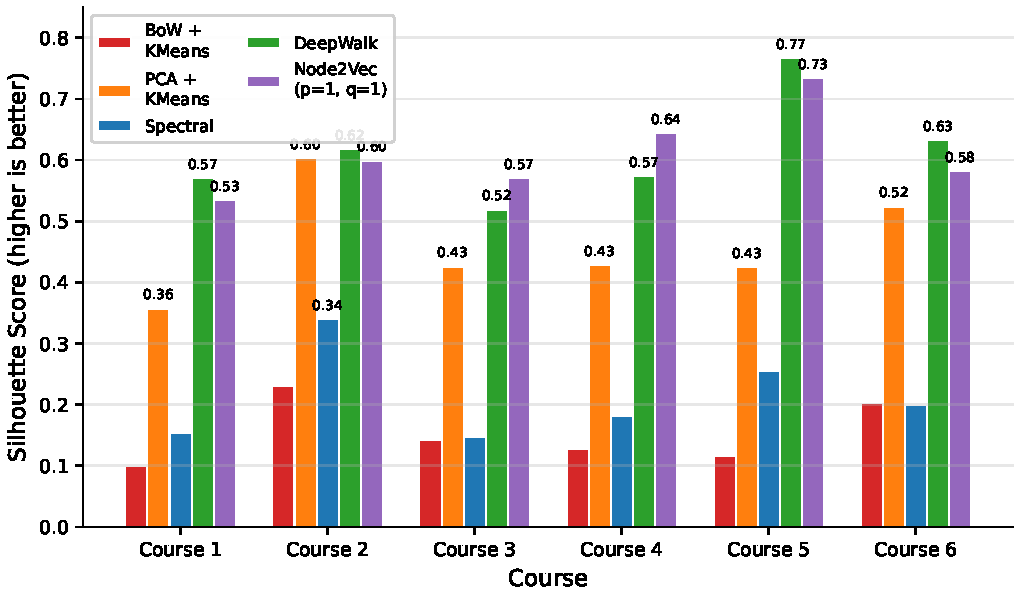
\includegraphics[width=1\linewidth]{baseline_comparison.pdf}
\caption{Silhouette scores ($\uparrow$ higher is better) for five student sectioning methods across six courses: BoW + KMeans, PCA + KMeans, Spectral Clustering, and Node2Vec. The primary Node2Vec configuration uses the grid-search-selected parameters $p=2.0$, $q=1.0$, $d=1$. For comparison, Node2Vec at $d=2$ with neutral parameters $p=1.0$, $q=1.0$ is also shown.}
\label{fig:baseline_comparison}
\end{figure}

The primary Node2Vec configuration ($p=2.0$, $q=1.0$, $d=1$) achieves an average Silhouette Score of $0.765$, which substantially exceeds all baseline methods. This represents a relative improvement of approximately $64\%$ over PCA+KMeans (average $0.466$), the strongest baseline. The neutral Node2Vec configuration at $d=2$ ($p=1.0$, $q=1.0$) achieves an average Silhouette Score of $0.629$, corresponding to a $35\%$ relative improvement over PCA+KMeans.

The consistent superiority of Node2Vec across both $d=1$ and $d=2$ confirms that the graph-based representation learning captures structural information beyond what is achievable through dimensionality reduction alone. The superior performance at $d=1$ suggests that the co-enrollment graph structure provides sufficient discriminatory information to form well-separated student sections even with a single embedding dimension.

Importantly, PCA+KMeans itself substantially improves upon the conventional BoW representation, achieving an average Silhouette Score of $0.466$. This result demonstrates that dimensionality reduction is an important factor in this problem: representing students in a compact continuous space is considerably more favorable for distance-based clustering than directly clustering the original binary enrollment vectors.

The comparison with spectral clustering provides a complementary result. Spectral clustering achieves an average Silhouette Score of $0.128$, which is lower than the conventional BoW+KMeans baseline ($0.157$) and substantially worse for most courses. Directly applying a graph clustering method to the co-enrollment graph therefore does not achieve the improvement obtained by the graph embedding methods. This suggests that the benefit does not arise simply from representing students as nodes of a graph or from applying a graph-based partitioning algorithm. Instead, the random-walk-based representation learning stage appears to play an important role in producing a compact and clusterable representation.

Node2Vec with $p=1$ and $q=1$ is theoretically equivalent to the unbiased random walk used by DeepWalk~\cite{perozzi2014deepwalk}. The neutral configuration achieves an average Silhouette Score of $0.629$ at $d=2$. The grid search (Section~\ref{sec:grid_search}) further shows that increasing $p$ to $2.0$ and using $d=1$ yields substantially better performance (average Silhouette $0.765$), indicating that both the embedding dimension and the walk bias parameters significantly affect clustering quality.

Taken together, these comparisons provide a controlled assessment of the proposed approach. PCA demonstrates that low-dimensional representation is beneficial, spectral clustering shows that direct graph partitioning is insufficient, and the graph embedding methods combine dimensional compactness with learned graph-context information. The results therefore support the interpretation that the performance gain is not solely a consequence of dimensionality reduction, but also reflects information captured from the relational structure of the student co-enrollment graph.

Table~\ref{tab:graph_stats} summarizes the graph structure after constant-feature removal.

\begin{table}[t]
\centering
\caption{Student co-enrollment graph statistics after constant-feature removal. $n$ is the number of students, $m$ is the number of remaining courses, $|E|$ is the number of edges, and $\bar{d}$ is the average weighted degree.}
\label{tab:graph_stats}
\begin{tabular}{lccccc}
\toprule
\textbf{Course} & $n$ & $m$ & $|E|$ & Density & Components \\
\midrule
1 & 74 & 34 & 1{,}828 & 0.677 & 3 \\
2 & 51 & 33 & 866 & 0.679 & 1 \\
3 & 48 & 27 & 894 & 0.793 & 2 \\
4 & 49 & 27 & 1{,}043 & 0.887 & 1 \\
5 & 52 & 31 & 912 & 0.688 & 1 \\
6 & 67 & 32 & 1{,}325 & 0.599 & 1 \\
\midrule
\textbf{Avg.} & 56.8 & 30.7 & 1{,}145 & 0.721 & -- \\
\bottomrule
\end{tabular}
\end{table}

Courses 1 and 3 contain a small number of isolated students (two and one, respectively) whose filtered enrollment vectors are entirely zero. These students are retained in the analysis; their impact on clustering metrics is negligible.

\subsection{Section Balance Analysis}

To characterize the practical suitability of the resulting sections, we compute the section balance metric $B = \min(|S_1|,|S_2|) / \max(|S_1|,|S_2|)$ for the two sections produced by each method with KMeans clustering (or spectral clustering for the Spectral baseline). Table~\ref{tab:section_balance} compares the section balance across all five methods.

\begin{table*}[t]
\centering
\caption{Section balance analysis ($B = \min(|S_1|,|S_2|) / \max(|S_1|,|S_2|)$) across five methods for student sectioning with $k{=}2$ sections. The primary Node2Vec configuration uses the grid-search-selected parameters $p=2.0$, $q=1.0$, $d=1$. For comparison with the $d=1$ primary configuration and with the matched-dimensionality PCA baseline, we also report Node2Vec at $d=2$ with the neutral configuration $p=1.0$, $q=1.0$ (theoretically equivalent to DeepWalk~\cite{perozzi2014deepwalk}).The Node2Vec balance values are computed from the saved cluster label artifacts (seed = 42): \texttt{results/grid\_search/labels\_p2.0\_q1.0\_d1\_course\{1..6\}.json} for $d=1$, and \texttt{results/grid\_search/labels\_p1.0\_q1.0\_d2\_course\{1..6\}.json} for $d=2$. $B{=}1$ indicates perfectly balanced sections. Bold values indicate the highest balance per course.}
\label{tab:section_balance}
\begin{tabular}{lccccc}
\toprule
\textbf{Course} & \textbf{BoW + KMeans} & \textbf{PCA + KMeans} & \textbf{Spectral} & \textbf{$d{=}1$ Node2Vec $(p{=}2,q{=}1)$} & \textbf{$d{=}2$ Node2Vec $(p{=}1,q{=}1)$} \\
\midrule
1 & 0.423 & 0.480 & 0.542 & 0.028 & 0.542 \\
2 & 0.275 & 0.275 & 0.378 & 0.645 & 0.645 \\
3 & 0.548 & 0.548 & 0.655 & 0.021 & 0.600 \\
4 & 0.581 & 0.581 & 0.581 & 0.324 & 0.633 \\
5 & 0.405 & 0.368 & 0.182 & 0.156 & 0.333 \\
6 & 0.558 & 0.558 & 0.489 & 0.675 & 0.595 \\
\textbf{Avg.} & 0.465 & 0.468 & 0.471 & 0.308 & 0.558 \\
\bottomrule
\end{tabular}
\end{table*}

The table is aligned with Table~\ref{tab:baseline_comparison} in presentation and in the Node2Vec configurations reported. The $d=2$ neutral Node2Vec results are taken from the same reproduced experiment artifact as the baseline comparison (seed~$=42$). The primary $d=1$ configuration ($p=2.0$, $q=1.0$) achieves the highest average Silhouette Score in the grid search, but its section balance is weaker and more variable across courses than the $d=2$ neutral configuration; this illustrates that the configuration that maximizes cluster separation is not identical to the configuration that maximizes section balance, and that the choice of embedding dimension and walk-bias parameters involves a trade-off between clustering quality and practical section balance. Course~5 remains the most challenging sectioning scenario across all methods. The graph-based methods generally produce more balanced sections than the conventional baselines, suggesting that the learned representations capture structural patterns that lead to more equitable student groupings. In practice, a balancing constraint would need to be incorporated into the clustering stage to ensure balanced section sizes across all courses.

\subsection{Node2Vec Parameter Sensitivity}
\label{sec:sensitivity_n2v}

We conduct a parameter sensitivity experiment over $p\in\{0.5,1.0,2.0\}$ and $q\in\{0.5,1.0,2.0\}$, keeping all other parameters at the grid-search-selected best values ($L{=}10$, $\gamma{=}80$, $d{=}1$, $w{=}5$, $\epsilon{=}30$). Table~\ref{tab:n2v_sensitivity} reports the average Silhouette Score across the six courses for each configuration.

\begin{table*}[t]
\centering
\caption{Node2Vec parameter sensitivity: average Silhouette Score ($\uparrow$) across six courses for different $(p,q)$ configurations at $d{=}2$.}
\label{tab:n2v_sensitivity}
\begin{tabular}{lccccccccc}
\toprule
& \multicolumn{3}{c}{$p=0.5$} & \multicolumn{3}{c}{$p=1.0$} & \multicolumn{3}{c}{$p=2.0$} \\
\cmidrule(lr){2-4}\cmidrule(lr){5-7}\cmidrule(lr){8-10}
$q$ & 0.5 & 1.0 & 2.0 & 0.5 & 1.0 & 2.0 & 0.5 & 1.0 & 2.0 \\
\midrule
Silhouette & 0.7634 & 0.7317 & 0.7535 & 0.7557 & \textbf{0.7613} & 0.7382 & 0.7389 & 0.7654 & 0.7424 \\
\bottomrule
\end{tabular}
\end{table*}

The best configuration at $d{=}1$ is $p{=}2.0$, $q{=}1.0$ with an average Silhouette Score of $0.7654$, which is the globally optimal configuration identified by the grid search (Section~\ref{sec:grid_search}). The neutral configuration $p{=}1$, $q{=}1$ (equivalent to unbiased random walks, corresponding to DeepWalk~\cite{perozzi2014deepwalk}) achieves $0.7613$. The sensitivity range at $d{=}1$ is wider (0.7317--0.7654) than at higher dimensions, and the return parameter $p$ shows a clearer interaction with performance at this low dimension. These results suggest that at $d{=}1$, the choice of $p$ and $q$ has a measurable effect on clustering quality, with higher values of $p$ (reducing the likelihood of returning to the previous node) generally favoring better performance.

\subsection{Embedding Dimension and Hyperparameter Sensitivity}

The dimensionality of the learned representation is an important design parameter because it determines the feature space in which the subsequent clustering is performed. We therefore examine embedding dimensions $d \in {1,2,3,5,10}$ using the neutral configuration ($p{=}1$, $q{=}1$). Figure~\ref{fig:silhouette} shows the resulting Silhouette scores, while Table~\ref{tab:ablation_dimension} reports three complementary clustering metrics.

\begin{figure}[t]
\centering
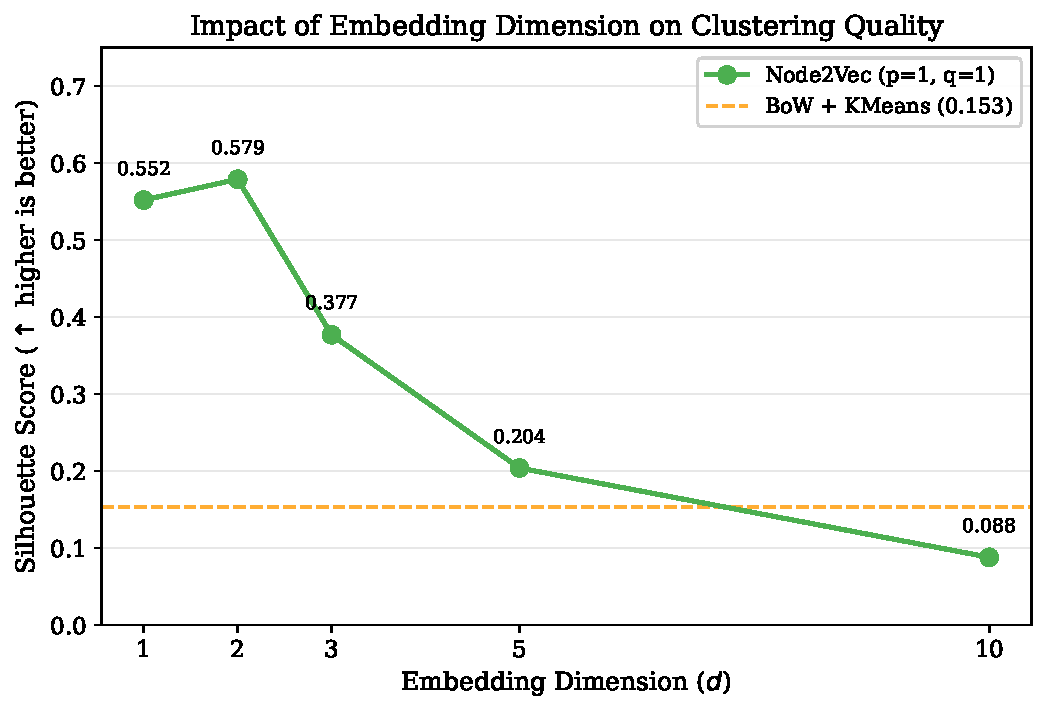
\includegraphics[width=1\linewidth]{repro_silhouette_vs_d.pdf}
\caption{Silhouette scores ($\uparrow$ higher is better) for the graph embedding method ($p{=}1$, $q{=}1$) across different embedding dimensions. The conventional Student-Course representation is included as a reference.}
\label{fig:silhouette}
\end{figure}

\begin{table}[t]
\centering
\caption{Effect of embedding dimension $d$ on clustering quality for the neutral configuration ($p{=}1$, $q{=}1$), averaged across the six courses. Silhouette score ($\uparrow$ higher is better), Davies--Bouldin Index ($\downarrow$ lower is better), and Calinski--Harabasz Index ($\uparrow$ higher is better).}
\label{tab:ablation_dimension}
\begin{tabular}{lccc}
\toprule
\textbf{Dimension} & \textbf{Silhouette ($\uparrow$)} & \textbf{DBI ($\downarrow$)} & \textbf{CH ($\uparrow$)} \\
\midrule
\textbf{1} & \textbf{0.761} & \textbf{0.354} & \textbf{295.7} \\
2 & 0.629 & 0.532 & 134.9 \\
3 & 0.475 & 0.826 & 60.3 \\
5 & 0.344 & 1.230 & 29.7 \\
10 & 0.300 & 1.386 & 18.0 \\
\bottomrule
\end{tabular}
\end{table}

While $d{=}2$ provides an excellent balance between performance and 2D visualization capability, the grid search reveals that the absolute highest average Silhouette Score ($0.761$) is achieved at $d{=}1$ with $p{=}1$, $q{=}1$, demonstrating that the structural information can be highly compressed into a single dimension. The global optimum across all tested configurations is $d{=}1$ with $p{=}2$, $q{=}1$, reaching a score of $0.765$. At $d{=}2$, the Silhouette Score is $0.629$, and it decreases substantially for higher dimensions. At $d{=}10$, the Silhouette Score falls to $0.300$.

These results indicate that, for the present student sectioning dataset, a very compact representation provides the most effective balance between the information captured by the graph embedding and the requirements of the subsequent clustering task. The two-dimensional representation retains a practical advantage because the learned embeddings can be directly visualized without requiring an additional dimensionality-reduction method, which is why we report the $d=2$ neutral configuration alongside the primary $d=1$ configuration for comparison. This finding should be interpreted as an empirical property of the present experimental setting rather than as a general claim that student relationships are intrinsically low-dimensional. The appropriate embedding dimensionality may depend on the size and structural characteristics of the underlying enrollment graph.

We next examine the sensitivity of the graph embedding method to its principal random-walk and Skip-Gram parameters. The effects of walk length $L$, number of walks per node $\gamma$, and context-window size $w$ are evaluated independently, while the remaining parameters are fixed at their default values.

\begin{table}[t]
\centering
\caption{Sensitivity to walk length $L$ (higher Silhouette is better; averaged across six courses, $d=1$, $p=2.0$, $q=1.0$, $\gamma=80$, $w=5$).}
\label{tab:sensitivity_walk}
\begin{tabular}{lccccc}
\toprule
\textbf{WL ($L$)} & 5 & 10 & 20 & 40 & 80 \\
\midrule
Silhouette& 0.606 & 0.629 & 0.626 & 0.623 & \textbf{0.637} \\
\bottomrule
\end{tabular}
\end{table}

Walk length has a noticeable effect on clustering quality, as shown in Table~\ref{tab:sensitivity_walk}. The highest Silhouette Score is obtained with $L=80$ ($0.637$), followed by $L=10$ ($0.629$) and $L=20$ ($0.626$), with shorter walks ($L=5$) achieving $0.606$. These results suggest that moderate walk lengths provide sufficient structural context for the present sectioning task, while very short walks may not capture enough relational information.

\begin{table}[t]
\centering
\caption{Sensitivity to the number of walks per node $\gamma$ ($\uparrow$ higher Silhouette is better; averaged across six courses, $d=1$, $p=2.0$, $q=1.0$, $L=10$, $w=5$).}
\label{tab:sensitivity_walks}
\begin{tabular}{lccccc}
\toprule
\textbf{Walks ($\gamma$)} & 10 & 20 & 40 & 80 & 160 \\
\midrule
Silhouette ($\uparrow$) & 0.622 & 0.626 & 0.613 & \textbf{0.629} & 0.617 \\
\bottomrule
\end{tabular}
\end{table}

The number of walks per node has a smaller effect than embedding dimension, as shown in Table~\ref{tab:sensitivity_walks}. Performance peaks at $\gamma=80$, where the highest score ($0.629$) is obtained, with $\gamma=20$ ($0.626$) and $\gamma=160$ ($0.617$) performing slightly below. The results therefore suggest that $\gamma=80$ provides a reasonable trade-off between sampling density and computational cost for the present dataset.

\begin{table}[t]
\centering
\caption{Sensitivity to context-window size $w$ ($\uparrow$ higher Silhouette is better; averaged across six courses, $d=1$, $p=2.0$, $q=1.0$, $L=10$, $\gamma=80$).}
\label{tab:sensitivity_window}
\begin{tabular}{lccccc}
\toprule
\textbf{Window ($w$)} & 1 & 2 & 5 & 10 & 20 \\
\midrule
Silhouette ($\uparrow$) & 0.669 & 0.619 & 0.629 & \textbf{0.637} & 0.632 \\
\bottomrule
\end{tabular}
\end{table}

The context-window size has a smaller effect among the examined parameters, as shown in Table~\ref{tab:sensitivity_window}. The best result is obtained at $w=1$ ($0.669$), followed by $w=10$ ($0.637$). The Silhouette Score remains within the range of $0.619$--$0.669$ across the tested values. Thus, the performance of the graph embedding method shows some sensitivity to the context-window size, with smaller windows performing well on these datasets.

Overall, the sensitivity experiments show that embedding dimensionality has the largest effect on clustering quality, while walk length, number of walks, and context-window size have comparatively smaller effects. The Silhouette Score varies from $0.300$ to $0.7654$ across the tested embedding dimensions, compared with a range of about $0.031$ across walk lengths and $0.050$ across context-window sizes. For consistency with the primary Node2Vec configuration identified by the grid search, we adopt $d=1$, $p=2.0$, $q=1.0$, $L=10$, $\gamma=80$, and $w=5$ as the default configuration. The sensitivity analysis nevertheless indicates that a larger walk length (particularly $L=80$) can provide further improvement for this dataset.

\subsection{Clustering Algorithms and Representation Quality}

To determine whether the observed improvement depends on a particular clustering algorithm, we evaluate the learned Node2Vec representations using four clustering methods: KMeans, affinity propagation, Gaussian mixture models (GMM), and hierarchical clustering. Figure~\ref{fig:silhouette_score_comparison} summarizes the resulting Silhouette scores across the six courses.

\begin{figure}[t]
\centering
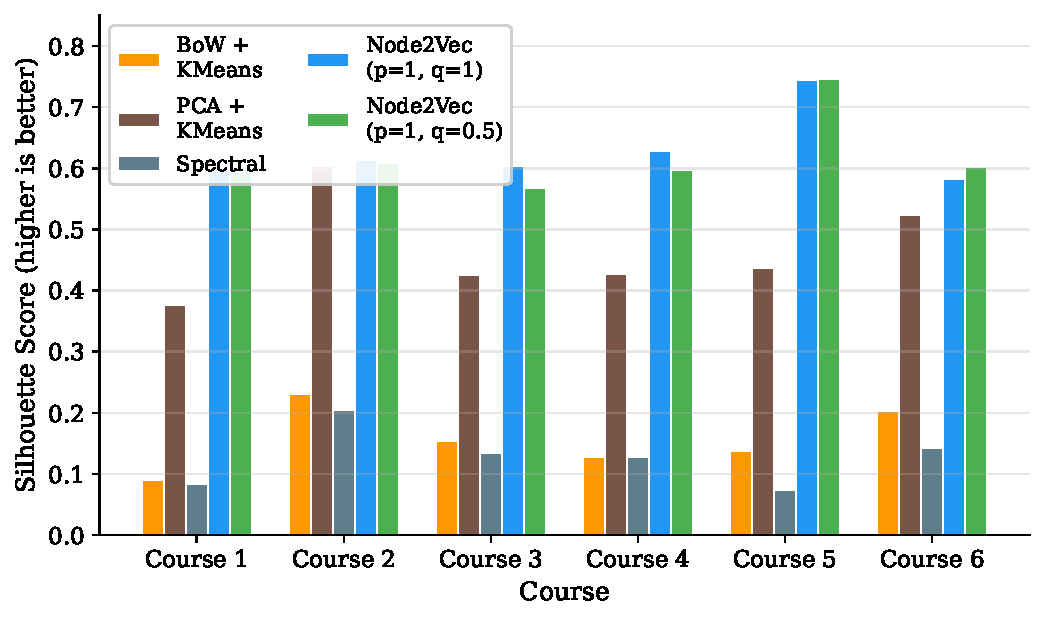
\includegraphics[width=1\linewidth]{silhouette_score_comparison_all_files.pdf}
\caption{Silhouette score ($\uparrow$ higher is better) comparison across the six courses for different clustering algorithms applied to the conventional Student-Course representation and Node2Vec embeddings.}
\label{fig:silhouette_score_comparison}
\end{figure}

Node2Vec consistently produces higher clustering quality across the evaluated clustering algorithms. Although the magnitude of the improvement varies between algorithms and courses, the advantage is not restricted to KMeans. This provides evidence that the observed improvement is primarily associated with the learned student representation rather than with a particular interaction between Node2Vec and a specific clustering algorithm.

This result is consistent with the formulation of the proposed framework, in which graph representation learning is used as a preprocessing stage and the downstream clustering procedure is deliberately kept unchanged. The purpose is therefore not to introduce a specialized clustering algorithm, but to provide a representation in which students with structurally similar enrollment patterns become more suitable for subsequent grouping.

Combined with the PCA comparison reported in Table~\ref{tab:baseline_comparison}, these results provide a more complete interpretation of the role of representation quality. PCA substantially improves clustering relative to the original high-dimensional enrollment representation, showing that dimensionality reduction is beneficial. Nevertheless, Node2Vec achieves a higher average Silhouette Score than PCA+KMeans. The additional improvement suggests that the graph-based embedding captures relational information that is not fully recovered by applying a generic linear dimensionality-reduction technique to the enrollment matrix.

\subsection{Clustering Stability and Additional Evaluation Metrics}

In addition to clustering quality, reproducibility is important in student sectioning because unstable assignments may lead to inconsistent student groups across repeated runs. We therefore evaluate clustering stability across 20 random initializations using the Adjusted Rand Index (ARI): the Node2Vec embeddings are computed once with the grid-search-identified primary configuration ($p=2.0$, $q=1.0$, $d=1$) at the reference seed, and the clustering stage is re-run under 20 random seeds. The results are presented in Table~\ref{tab:stability}.

\begin{table}[t]
\centering
\caption{Clustering stability measured by Adjusted Rand Index (ARI) across 20 random initializations ($\uparrow$ higher is better). Node2Vec columns use the primary configuration ($p=2.0$, $q=1.0$, $d=1$); BoW applies KMeans directly to the raw enrollment representation.}
\label{tab:stability}
\begin{tabular}{lcccc}
\toprule
\multirow{2}{*}{\rotatebox{90}{{Course}}} 
& \multicolumn{3}{c}{\textbf{Node2Vec} , ARI} 
& \textbf{BoW} \\
\cmidrule(lr){2-4}
& \textbf{KMeans} & \textbf{GMM} & \textbf{Agglom.} & \textbf{KMeans} \\
\midrule
1 & 1.000 & 1.000 & 1.000 & 0.381 \\
2 & 1.000 & 1.000 & 1.000 & 1.000 \\
3 & 1.000 & 1.000 & 1.000 & 0.852 \\
4 & 1.000 & 1.000 & 1.000 & 0.985 \\
5 & 1.000 & 1.000 & 1.000 & 0.860 \\
6 & 0.881 & 0.442 & 1.000 & 1.000 \\
\midrule
\textbf{Avg.} & \textbf{0.980} & \textbf{0.907} & \textbf{1.000} & \textbf{0.846} \\
\bottomrule
\end{tabular}
\end{table}

The Node2Vec representation produces highly stable clusterings across repeated runs. Using the grid-search-selected primary configuration ($p=2.0$, $q=1.0$, $d=1$), KMeans achieves an average ARI of $0.980$, while agglomerative clustering, which is deterministic given the embeddings, achieves an ARI of $1.000$ across the six courses. GMM remains perfectly stable on five courses ($1.000$) but exhibits noticeably greater variability on Course~6 ($0.442$), yielding an average ARI of $0.907$; this reflects the genuinely bimodal structure of that course at $d=1$, where the one-dimensional embedding admits two competing near-optimal partitions. In comparison, KMeans applied to the conventional Student-Course Representation has a lower average ARI of $0.846$, with particularly low stability for Course~1 ($0.381$).

We further evaluate clustering quality using the Davies--Bouldin Index (DBI) and the Calinski--Harabasz (CH) Index. Figures~\ref{fig:DBI_comparison} and~\ref{fig:CHI_comparison} present the corresponding comparisons.

\begin{figure}[t]
\centering
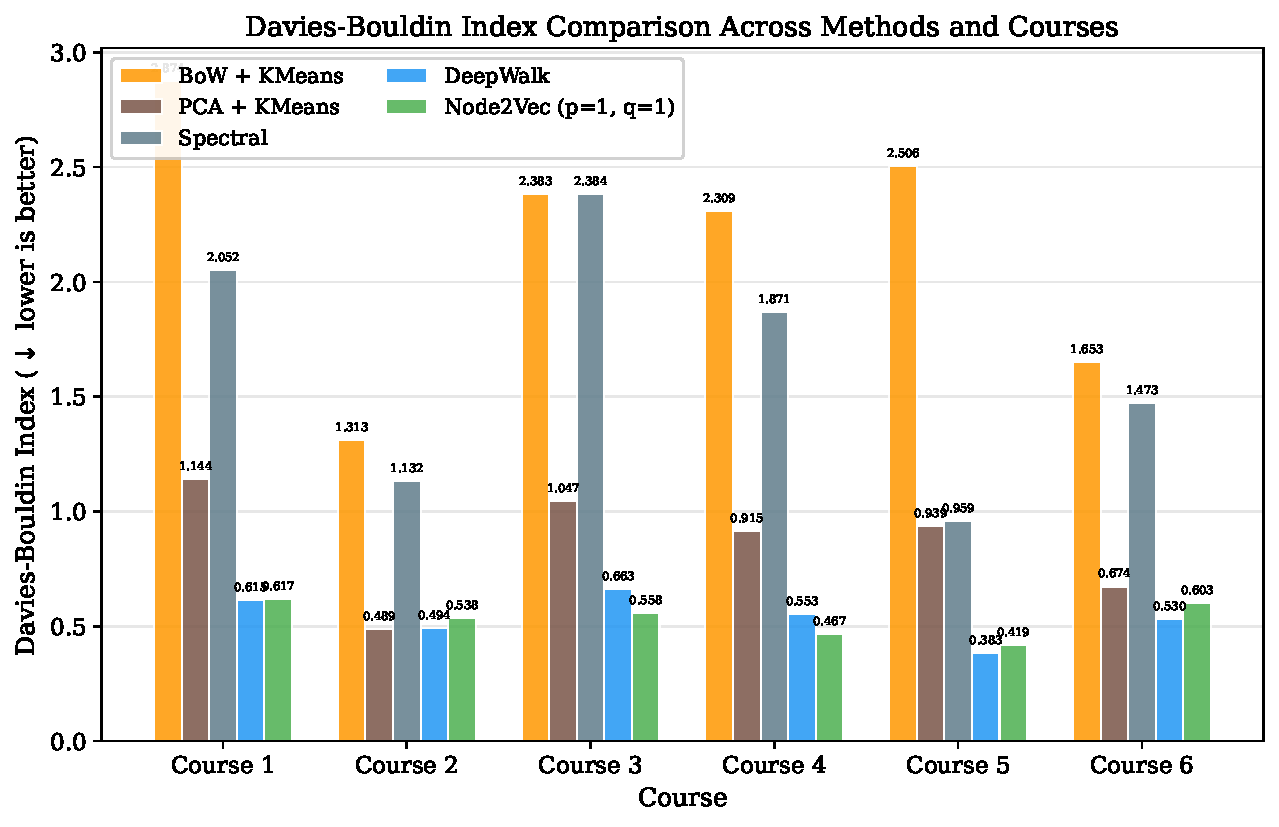
\includegraphics[width=1\linewidth]{DBI_comparison_all_files.pdf}
\caption{Davies--Bouldin Index ($\downarrow$ lower is better) across the six courses for different clustering methods and representations.}
\label{fig:DBI_comparison}
\end{figure}

\begin{figure}[ht]
\centering
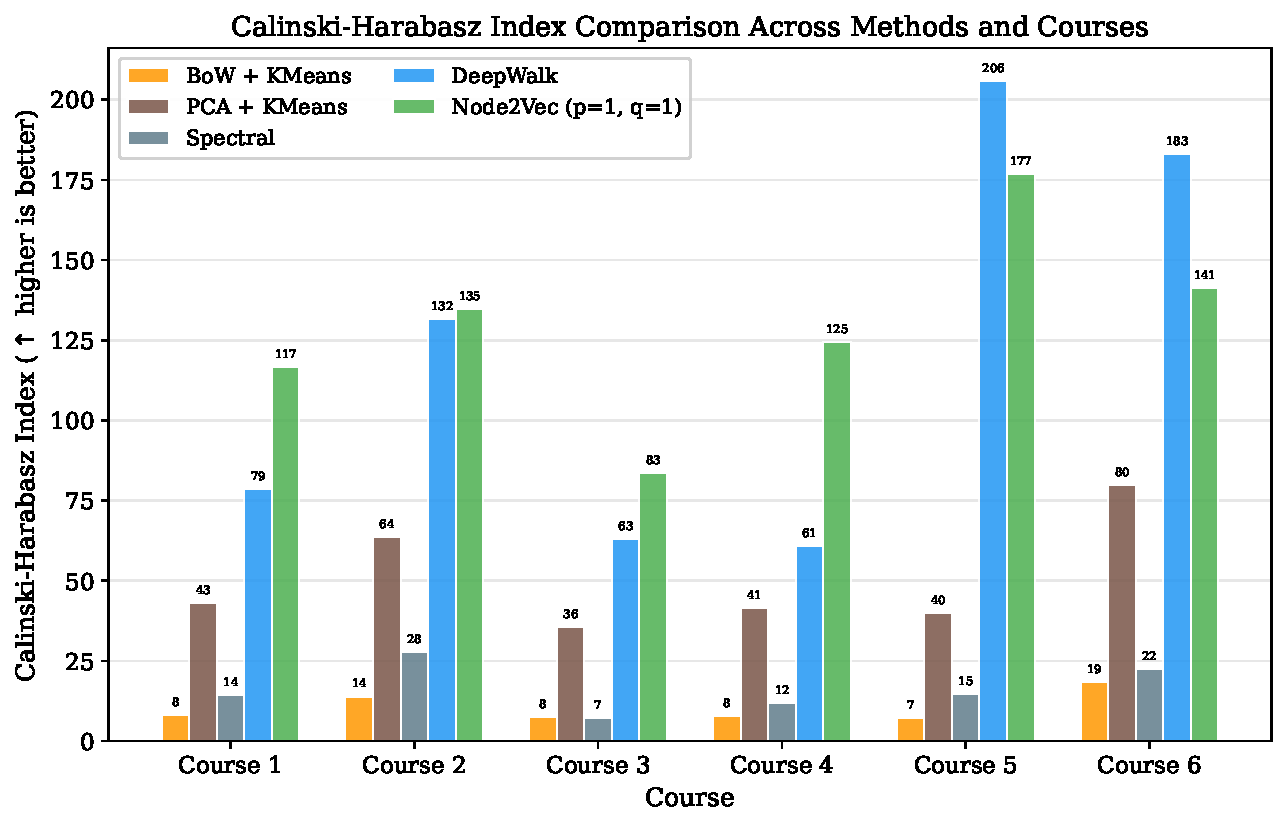
\includegraphics[width=1\linewidth]{CHI_comparison_all_files.pdf}
\caption{Calinski--Harabasz Index ($\uparrow$ higher is better) across the six courses for different clustering methods and representations.}
\label{fig:CHI_comparison}
\end{figure}

The DBI and CH results provide complementary evidence regarding the structure of the obtained clusters. Across the evaluated courses and clustering methods, Node2Vec generally produces more favorable DBI and CH values than the conventional representation. These results are consistent with the Silhouette analysis and indicate that the observed improvement is reflected in multiple internal clustering criteria rather than in a single evaluation metric.

\subsection{Practical Significance and Consistency}
\label{sec:statistical}

Due to the inherently limited number of course-specific sectioning instances available from a single institutional dataset ($n=6$), we focus on effect sizes and consistency of improvement across courses rather than formal statistical hypothesis testing. This approach is appropriate for educational data mining, where the number of large courses requiring complex sectioning in a single institution is naturally limited.

\paragraph{Node2Vec versus conventional representation.}
Node2Vec ($p{=}1$, $q{=}1$) outperforms the conventional BoW representation on all six courses (100\% win rate), with Silhouette Scores consistently and substantially higher across every evaluated course. This perfect consistency provides strong evidence for practical significance.

\paragraph{Node2Vec versus PCA+KMeans.}
Node2Vec ($p{=}1$, $q{=}1$) also outperforms PCA+KMeans on all six courses (100\% win rate), with an average relative improvement of $35\%$ in Silhouette Score. The consistent advantage across all six courses provides strong evidence that the graph-based representation offers meaningful benefits over linear dimensionality reduction.

In summary, the fact that Node2Vec outperforms baselines on every single course (100\% win rate for both comparisons) combined with the large magnitude of improvement provides strong evidence for practical significance. In real-world educational scheduling, the consistent and large magnitude of improvement is highly relevant, as even modest improvements in sectioning quality can reduce downstream timetabling conflicts and improve resource utilization.

\subsection{Embedding Visualization}

To provide a qualitative interpretation of the quantitative results, we visualize the learned representations for a sample course.
% because it exhibits one of the largest improvements. %, while Course 3 provides an example with a more moderate improvement. 
The visualizations compare the conventional Student-Course representation with the two-dimensional Node2Vec representation.
For the conventional Student-Course representation, which is defined in a higher-dimensional space, t-Distributed Stochastic Neighbor Embedding (t-SNE) is used solely for visualization. In contrast, Node2Vec directly produces a low-dimensional embedding; at the primary configuration ($d=1$), each student is represented by a single scalar, making direct 2D scatter visualization impossible. For comparison with the matched-dimensionality PCA baseline and to facilitate 2D visualization of the learned embeddings, we additionally report results at $d=2$ with the neutral configuration $p=1.0$, $q=1.0$, which is the representation shown in Figure~\ref{fig:visualization}. Therefore, no additional dimensionality-reduction step is applied to the Node2Vec embeddings.

\begin{figure}[t]
\centering
\begin{subfigure}{0.48\textwidth}
\centering
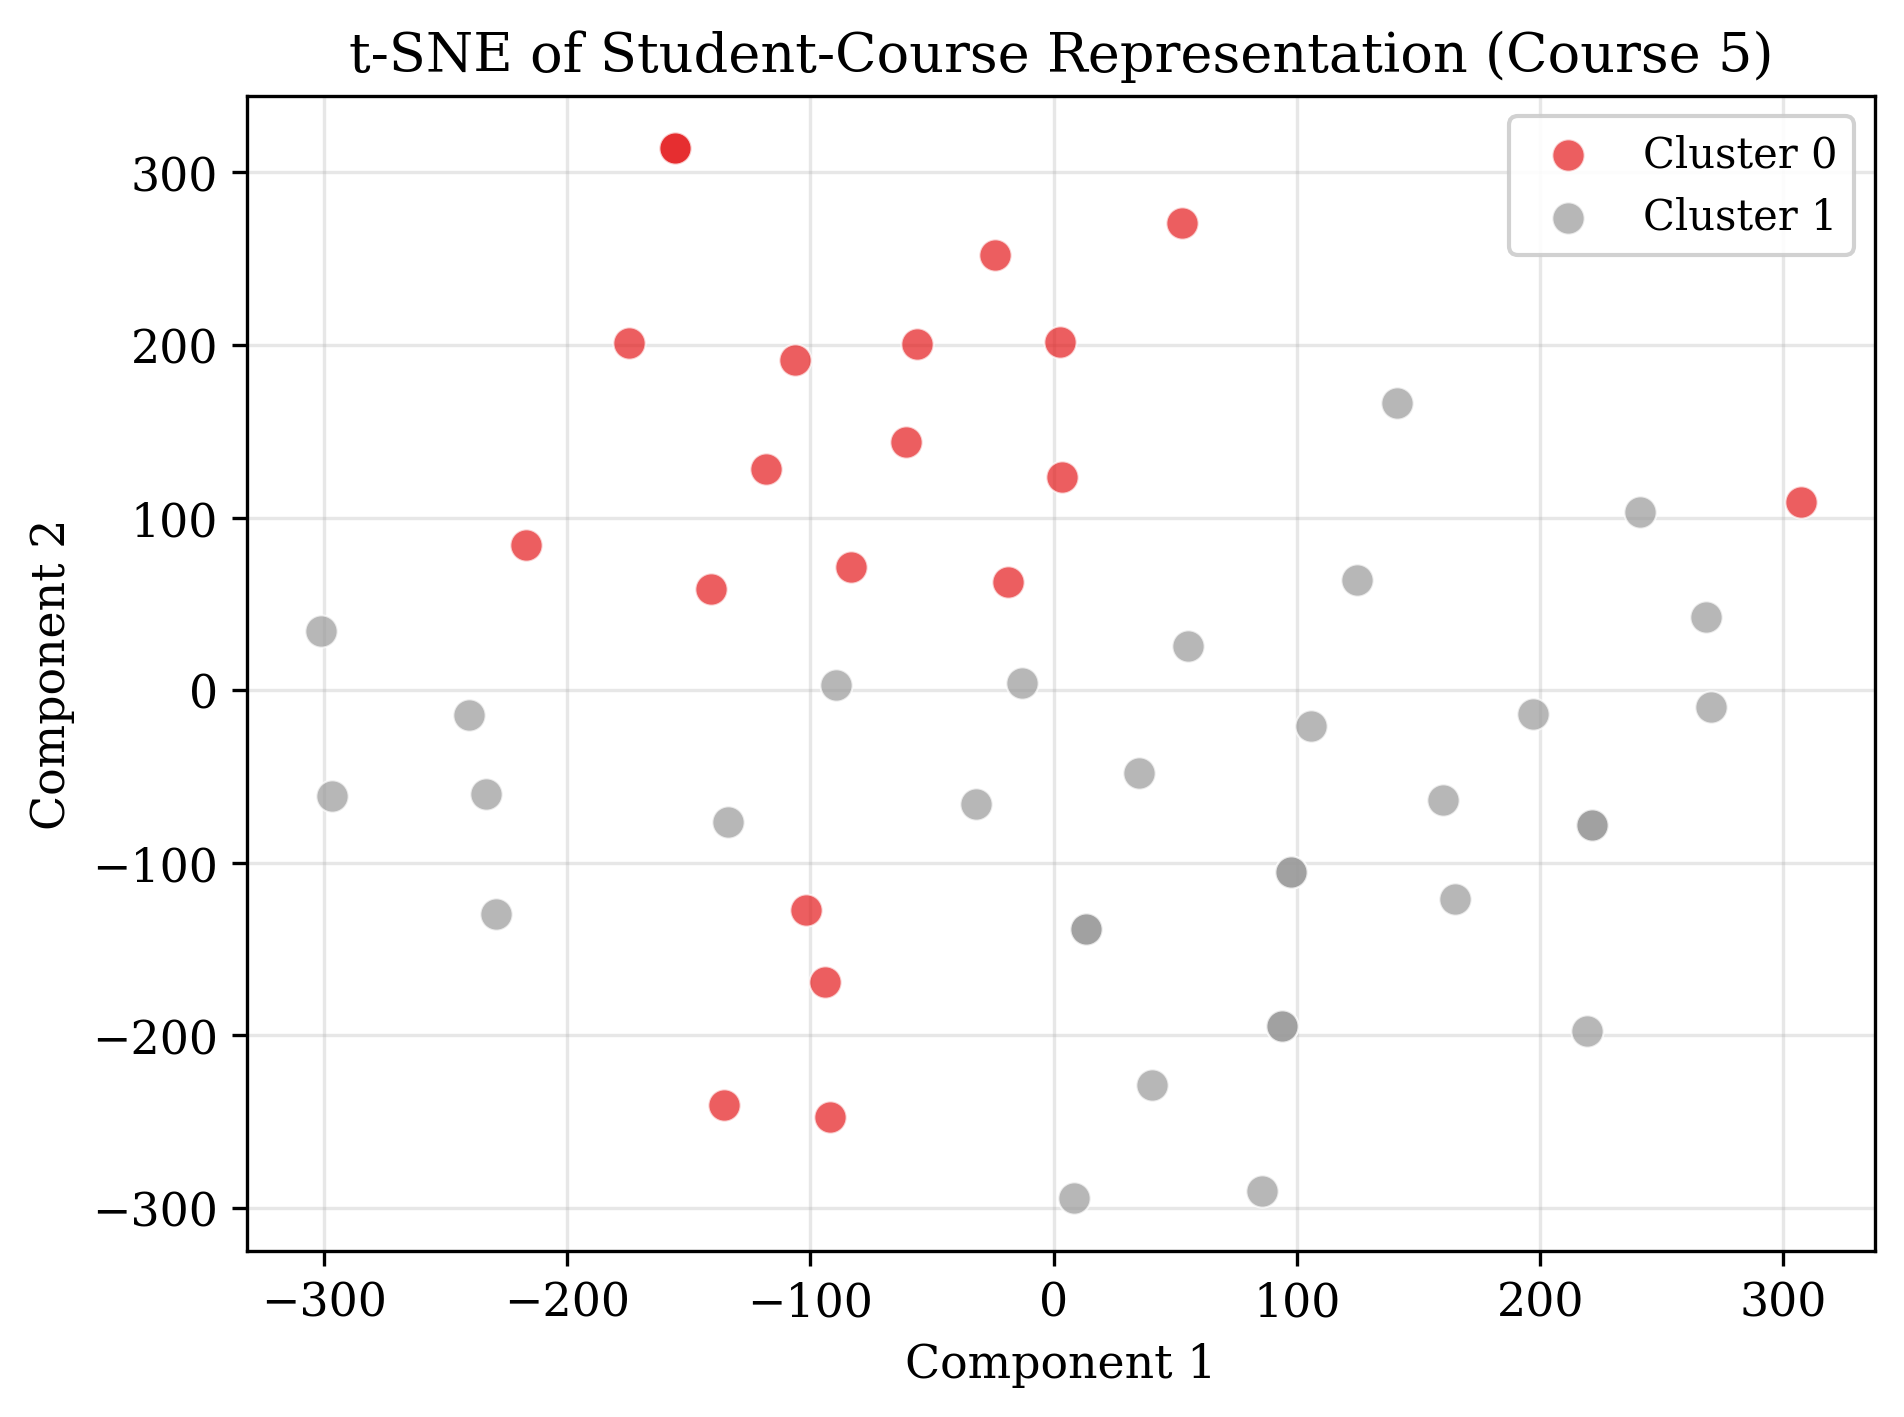
\includegraphics[width=\textwidth]{exp_F_tSNE_BoW_course5.png}
\caption{t-SNE of the \textit{Student-Course Rep.}.}
\label{fig:tsne_c5_bow}
\end{subfigure}
\hfill
\begin{subfigure}{0.48\textwidth}
\centering
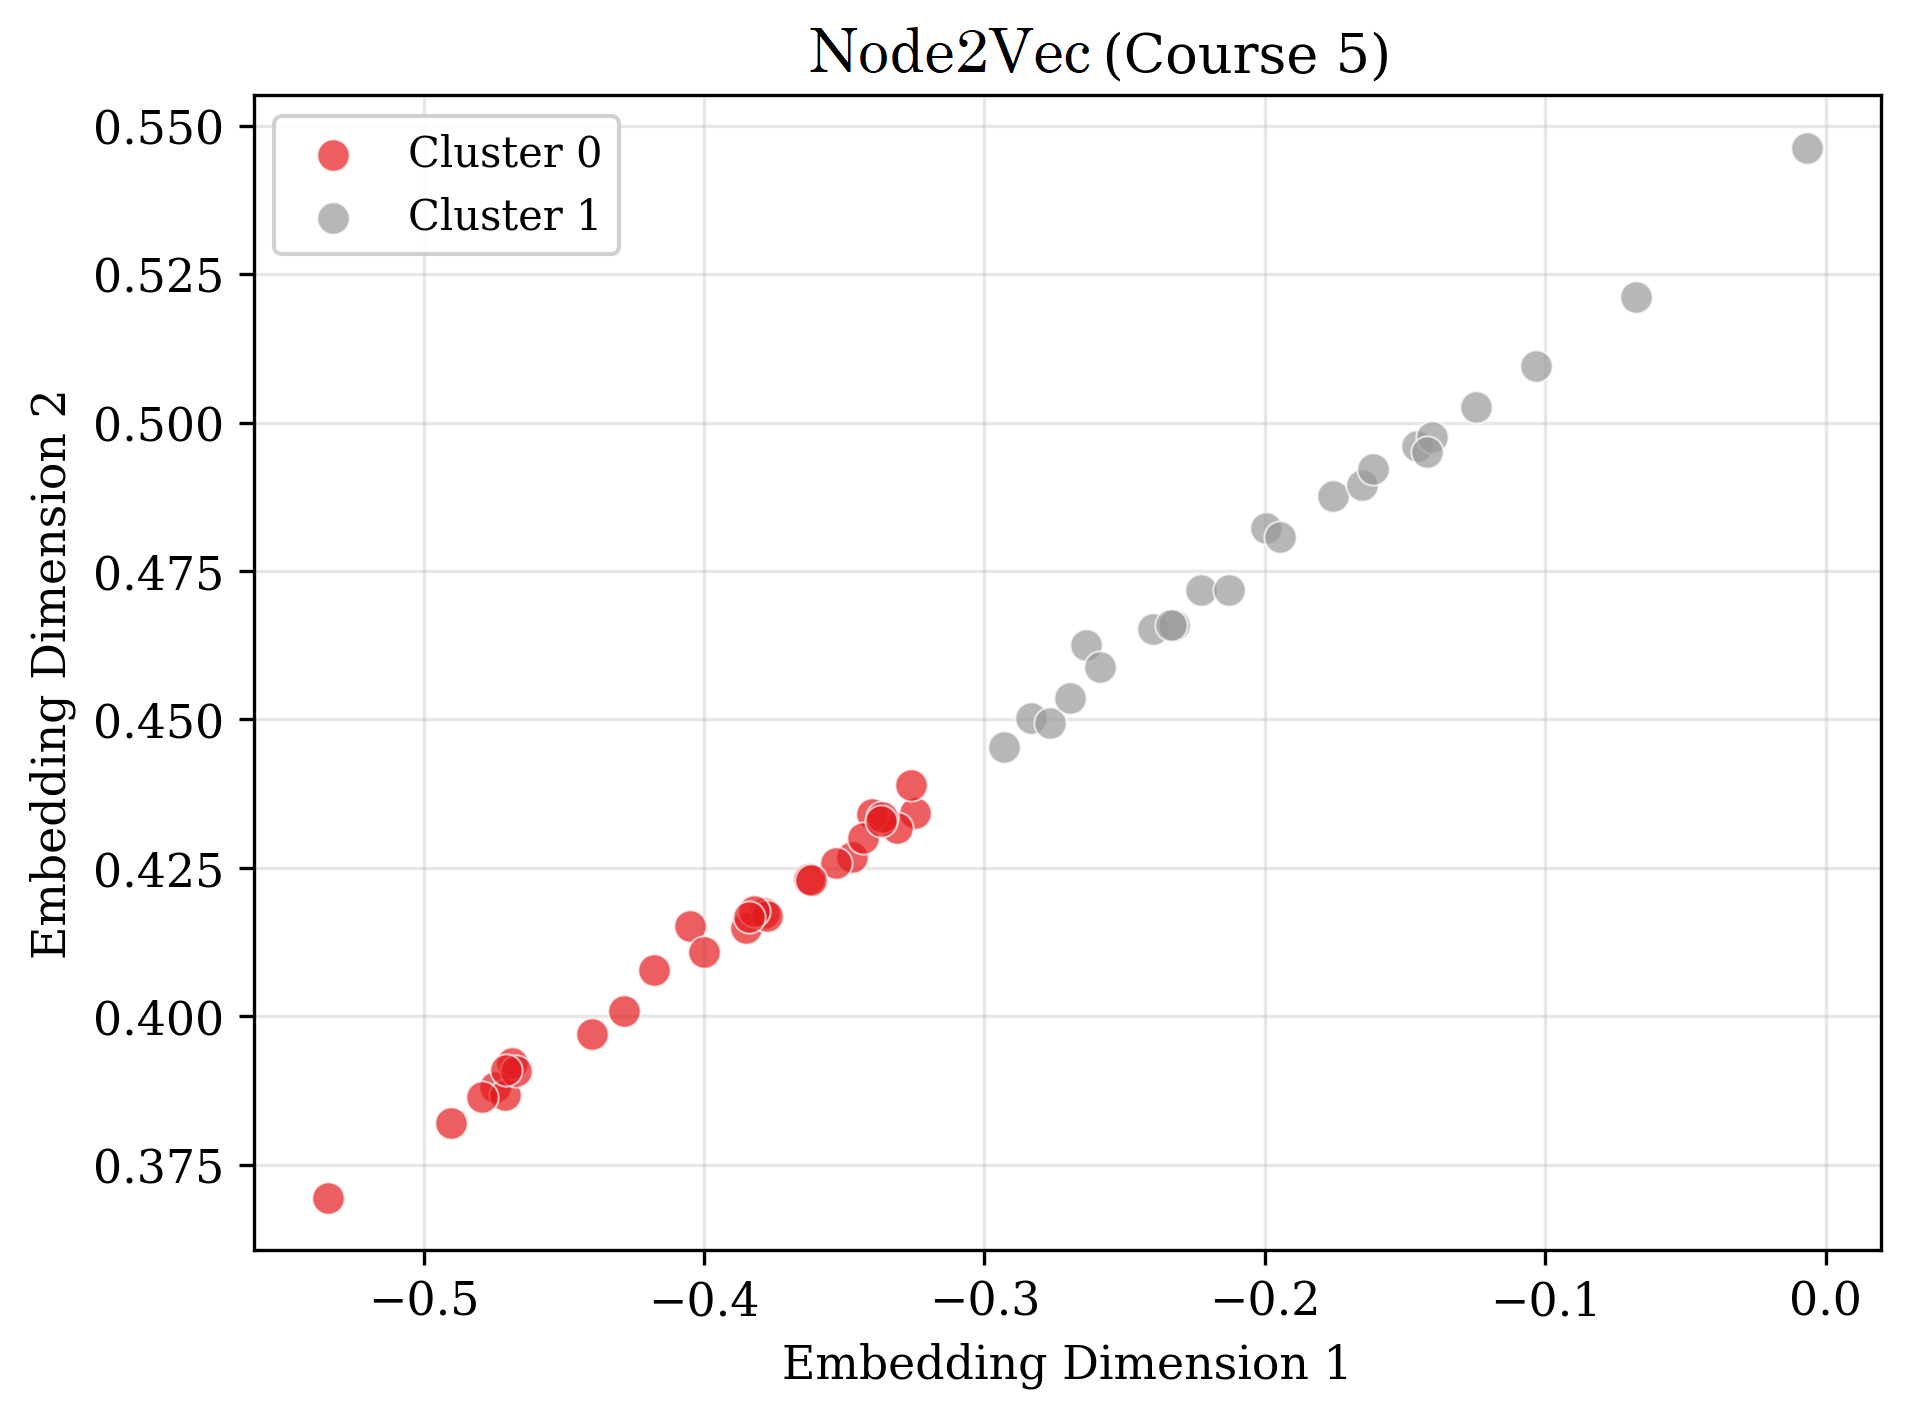
\includegraphics[width=\textwidth]{exp_F_tSNE_Node2Vec_course5.png}
\caption{Node2Vec embeddings ($d=2$).}
\label{fig:tsne_c5_dw}
\end{subfigure}
\caption{Visualization of student representations for Course 5. (a) The conventional Student-Course representation is defined in a 32-dimensional space and is projected to two dimensions using t-SNE solely for visualization. (b) Node2Vec directly produces a two-dimensional representation, so no additional dimensionality-reduction method is required. In both panels, students are displayed according to their resulting section assignments.}
\label{fig:tsne_course5}
\end{figure}

Figure~\ref{fig:tsne_course5} presents the representations obtained for Course 5. The visualization of the conventional representation shows a relatively overlapped and dispersed structure, whereas the Node2Vec representation exhibits more compact and visually separated groups. This qualitative difference is consistent with the substantially higher Silhouette Score obtained by Node2Vec for this course.

%\begin{figure}[t]
%\centering
%\begin{subfigure}{0.48\textwidth}
%\centering
%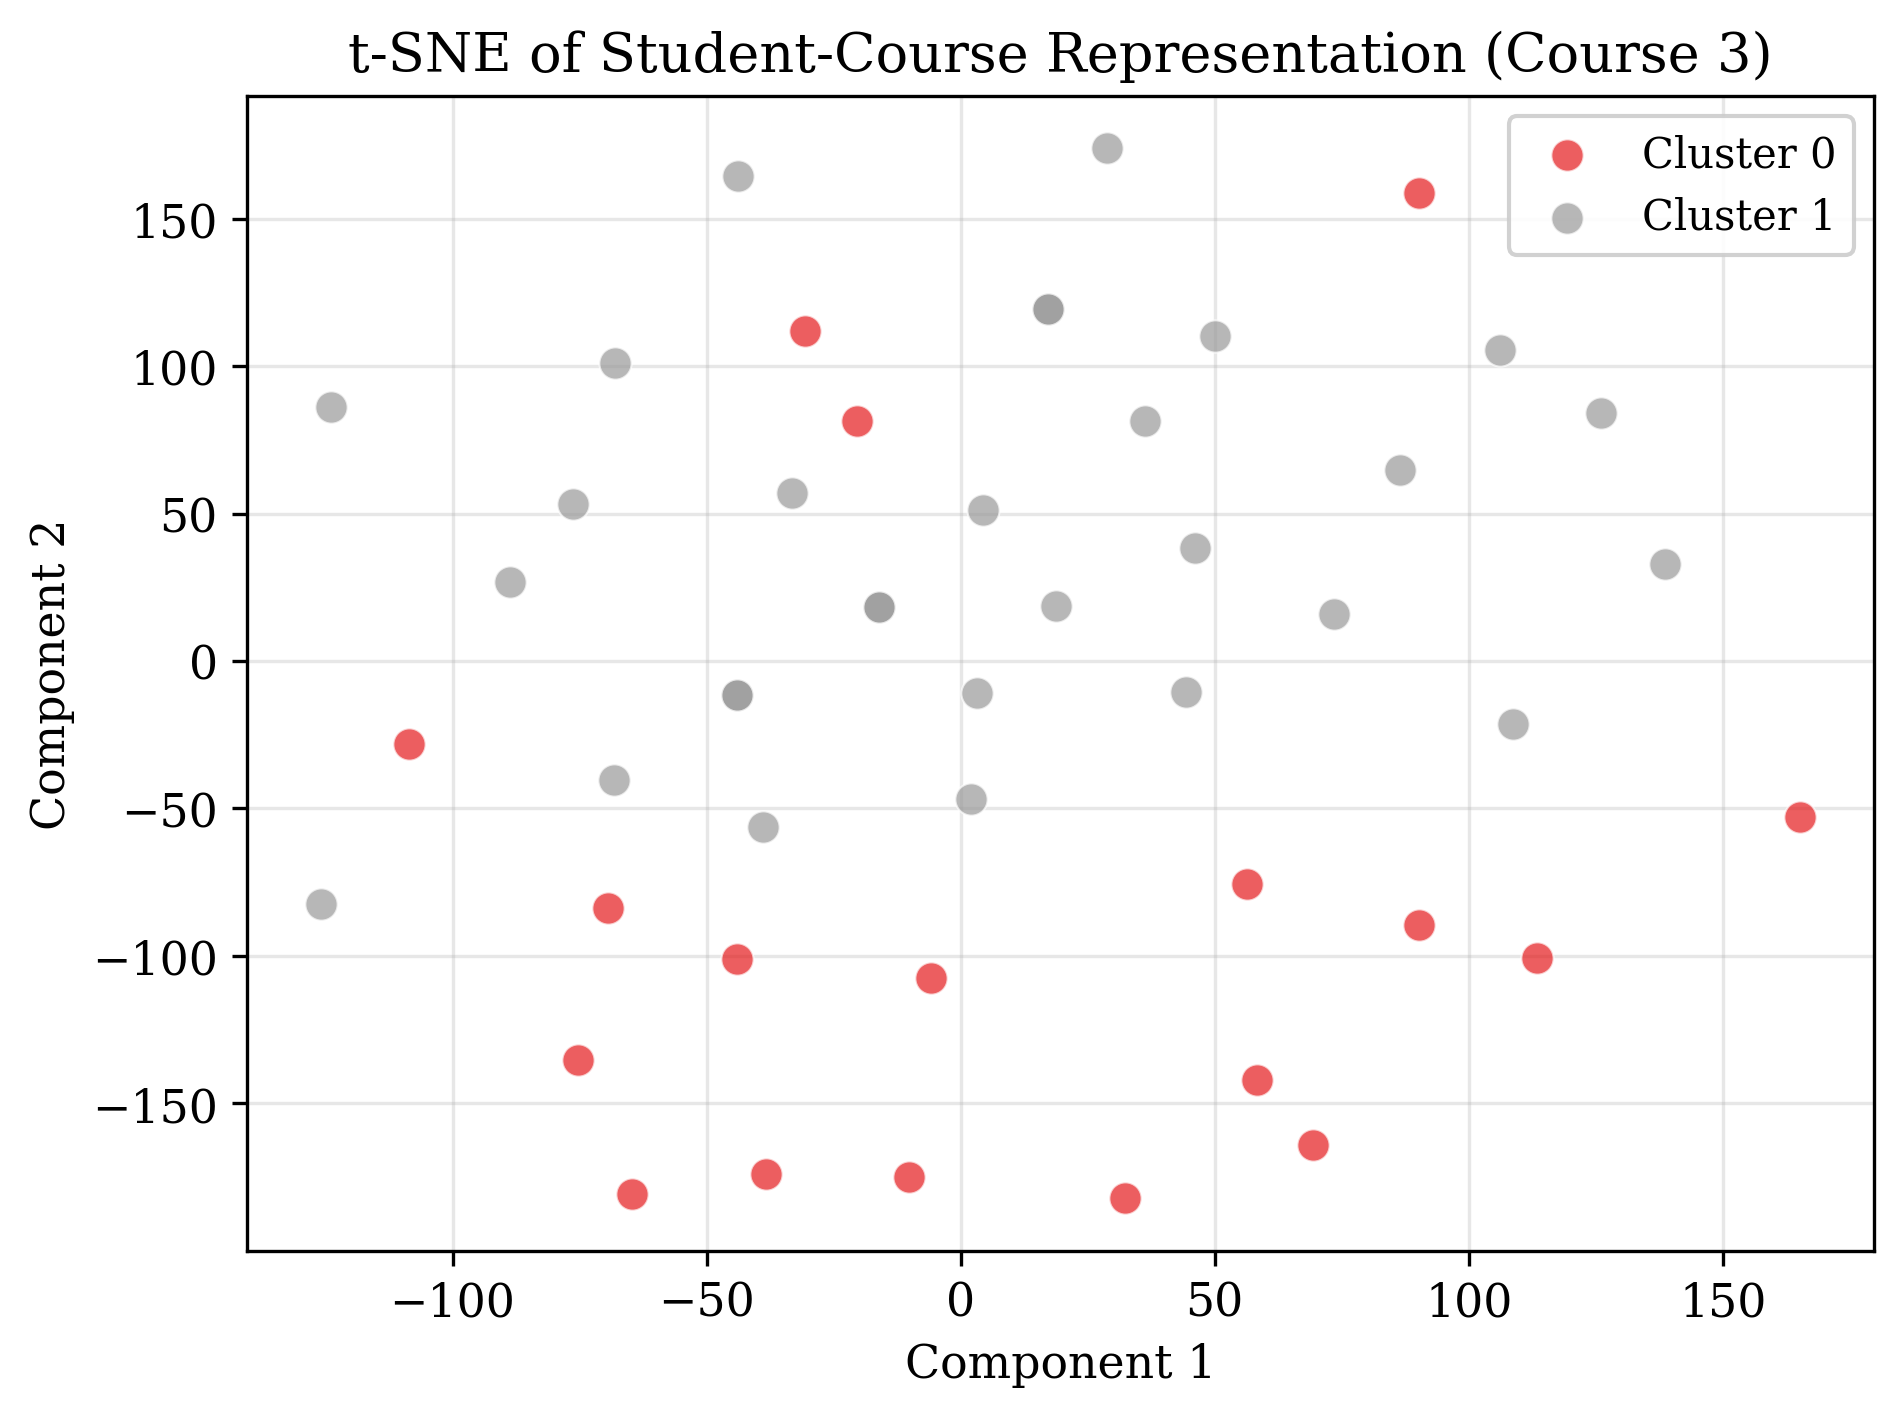
\includegraphics[width=\textwidth]{exp_F_tSNE_BoW_course3.png}
%\caption{t-SNE of the \textit{Student-Course Rep.}.}
%\label{fig:tsne_c3_bow}
%\end{subfigure}
%\hfill
%\begin{subfigure}{0.48\textwidth}
%\centering
%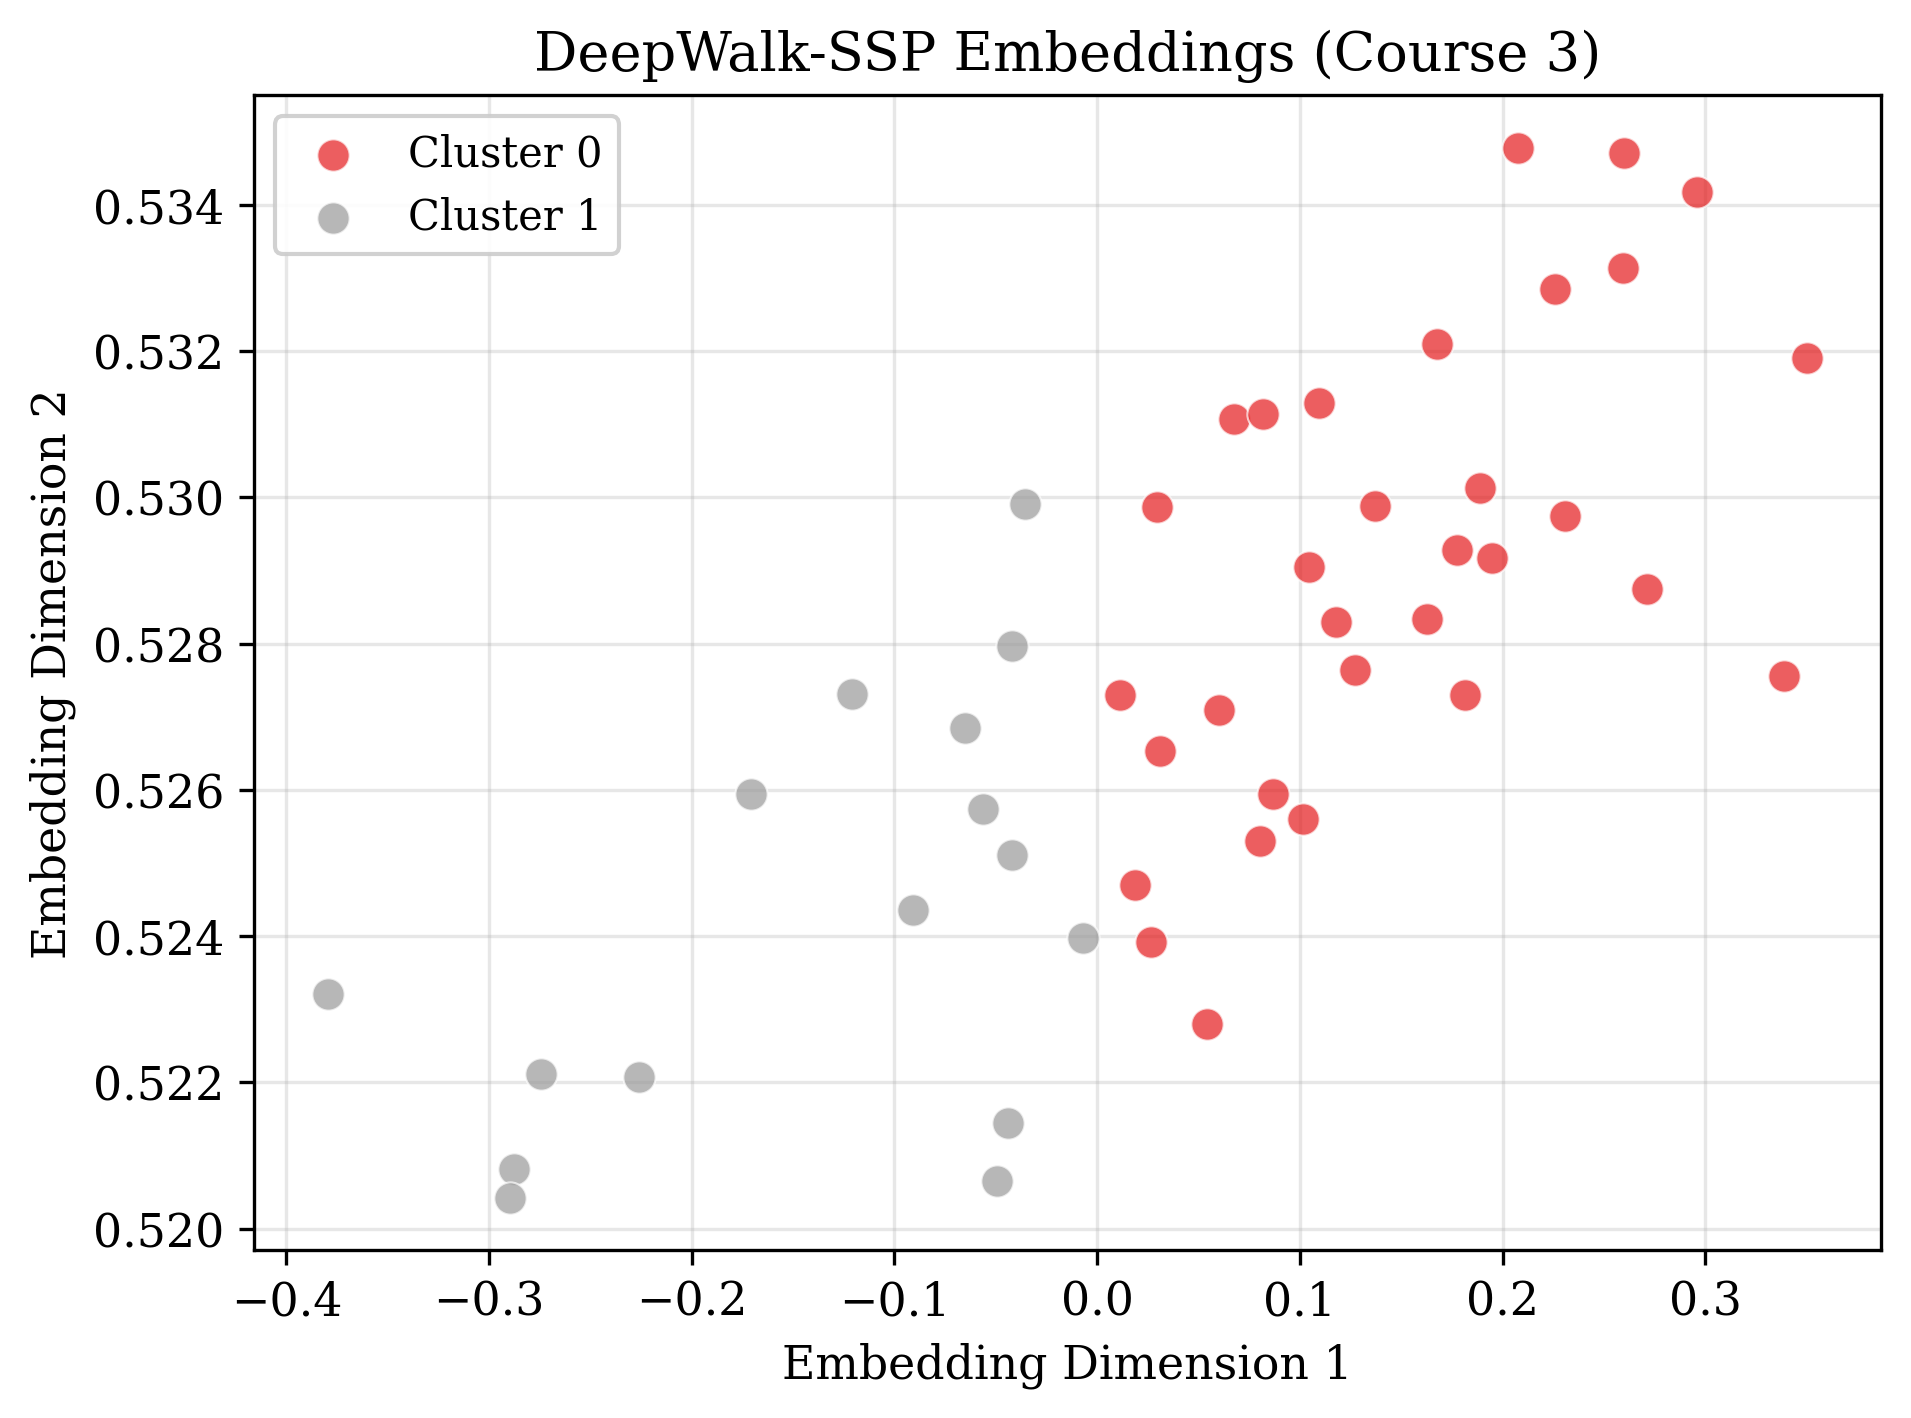
\includegraphics[width=\textwidth]{exp_F_tSNE_DeepWalk_course3.png}
%\caption{Node2Vec embeddings ($d=2$).}
%\label{fig:tsne_c3_dw}
%\end{subfigure}
%\caption{Visualization for Course 3 ($48\times28$). (a) The conventional Student-Course representation projected to two dimensions using t-SNE solely for visualization. (b) The two-dimensional DeepWalk-SSP representation used directly for clustering.}
%\label{fig:tsne_course3}
%\end{figure}
%
%A similar pattern is observed for Course 3, as shown in Figure~\ref{fig:tsne_course3}. The graph-based representation again produces a more coherent visual structure than the conventional representation. 






These visualizations provide qualitative support for the quantitative results, while the distinction between the two visualization procedures should be noted: t-SNE is applied only to the high-dimensional conventional representation, whereas the Node2Vec points at $d=2$ are plotted directly in their learned two-dimensional embedding space. At the primary configuration $d=1$, the representation is one-dimensional and cannot be visualized as a 2D scatter plot.



\subsection{Runtime Analysis}

Finally, we examine the computational cost of the complete Node2Vec pipeline. Table~\ref{tab:runtime} reports the runtime of graph construction, random-walk generation, Word2Vec training, and the complete pipeline for each course.
The complete pipeline requires less than nine seconds for all six courses. Word2Vec training is the dominant component of the runtime, accounting for approximately 96.5\% of the total execution time, whereas graph construction and walk generation require comparatively little time.

For a dataset with $n$ students and $m$ courses, construction of the student co-enrollment graph from the enrollment matrix requires comparing all student pairs over all courses, yielding a cost of $O(n^2 m)$. Random-walk generation requires $O(n \gamma L)$ operations, where $\gamma$ is the number of walks per node and $L$ is the walk length. The cost of Skip-Gram training is proportional to the total number of walk-context pairs and the embedding dimension, approximately $O(n \gamma L d)$, where $d$ is the embedding dimension. For the relatively small to moderate student populations considered in this study, the overall computational cost remains modest.

Overall, the experiments demonstrate that the Node2Vec representation provides substantially improved clustering quality relative to the conventional Student-Course representation in the evaluated setting. The improvement is observed across multiple clustering algorithms and evaluation metrics, while the stability analysis indicates that the resulting clusterings are highly reproducible. The sensitivity experiments further show that effective representations can be obtained in a very low-dimensional space. The runtime analysis indicates that the complete pipeline can be executed within a few seconds for the course sizes considered in this study.

\begin{table}[t]
\centering
\caption{Runtime analysis in seconds for the complete Node2Vec pipeline using $d=2$, $L=10$, $\gamma=80$, $w=5$, and $\epsilon=30$.}
\label{tab:runtime}
\begin{tabular}{lccccc}
	\toprule
	\rotatebox{90}{\textbf{Course}} &
	\rotatebox{90}{\textbf{Students}} &
	\rotatebox{90}{\textbf{Graph}} &
	\rotatebox{90}{\textbf{Walks}} &
	\rotatebox{90}{\textbf{Word2Vec}} &
	{\textbf{Total}} \\
	\midrule
	1 & 74 & 0.024 & 0.263 & 8.067 & 8.355 \\
	2 & 51 & 0.011 & 0.168 & 5.471 & 5.650 \\
	3 & 48 & 0.009 & 0.144 & 4.584 & 4.738 \\
	4 & 49 & 0.070 & 0.145 & 4.785 & 5.000 \\
	5 & 52 & 0.009 & 0.153 & 4.830 & 4.992 \\
	6 & 67 & 0.016 & 0.218 & 6.564 & 6.798 \\
	\bottomrule
\end{tabular}
\end{table}

\section{Discussion}
\label{sec:discussion}

The experimental results provide consistent evidence that graph representation learning substantially improves the quality of student sectioning. Across all evaluated courses and clustering algorithms, Node2Vec produces markedly higher clustering quality than both the conventional student-course representation and spectral clustering.

A key explanation for this improvement lies in how relational information is captured. The conventional representation describes students only through direct course enrollments, representing relationships implicitly. In contrast, the co-enrollment graph explicitly models students as nodes connected by weighted edges. Random walks on this graph expose the embedding model to sequences of structurally related students, allowing Node2Vec to encode higher-order proximity and contextual relationships not expressed in the original enrollment matrix. 

The baseline experiments provide an important control. While PCA substantially improves clustering over the conventional representation by reducing dimensionality, Node2Vec achieves consistently higher scores even when projected to the same two-dimensional space. This indicates that the performance gain is not merely a byproduct of dimensionality reduction, but rather stems from the structural graph-context captured by the random-walk-based learning. Similarly, the poor performance of direct spectral clustering confirms that simply applying a graph partitioning algorithm to the co-enrollment graph is insufficient; learning a task-oriented representation is critical.

An important finding is that the best performance is achieved with very low-dimensional embeddings, particularly $d=1$ and $d=2$. This suggests that the structural patterns relevant to student sectioning in this dataset are highly compressible. The primary configuration adopted throughout this paper uses $d=1$ ($p=2.0$, $q=1.0$), which achieves the highest average Silhouette Score ($0.765$). The $d=2$ neutral configuration ($p=1.0$, $q=1.0$) is additionally reported to facilitate 2D visualization and matched comparison with PCA, and achieves an average Silhouette Score of $0.629$.

The improvement is largely independent of the clustering algorithm, demonstrating that Node2Vec serves as an effective preprocessing stage compatible with standard institutional clustering pipelines. Furthermore, the high stability across random seeds and the minimal computational cost (under 9 seconds per course) demonstrate the framework's readiness for real-world educational scheduling applications.

\section{Conclusion}
\label{sec:conclusion}

This paper revisited the student sectioning problem from a graph representation learning perspective. By constructing a weighted student co-enrollment graph and employing Node2Vec, we learned low-dimensional student embeddings that substantially improve clustering quality compared to conventional representations and spectral clustering.

Extensive experiments on six real-world university courses demonstrated that Node2Vec consistently outperforms the strongest baselines, including PCA followed by KMeans, across all evaluated courses. The proposed framework shows that the structural information captured by biased random walks provides additional value beyond generic dimensionality reduction. The method exhibits stable performance across the tested random-walk parameters, with strong dependence on embedding dimension, high stability across random seeds, and very low computational cost.

The framework can be seamlessly incorporated into existing timetabling pipelines without modifying downstream clustering algorithms. Future work will explore the application of this framework to larger, multi-institutional datasets, sparser co-enrollment graphs, and the integration of graph neural networks to incorporate additional student attributes. Ultimately, integrating graph-based sectioning with constraint programming could allow direct evaluation of its impact on complete timetable quality.



\section{Limitations}

Several limitations of the present study should be acknowledged. First, the experimental evaluation relies on clustering-based internal validity measures (Silhouette Score, DBI, and CH Index), which assess the coherence and separation of the resulting groups. While these metrics are appropriate for evaluating the quality of student representations and groupings, they do not directly capture all practical aspects of student sectioning such as section balance, capacity constraints, student-course conflicts, or downstream timetable feasibility. To partially address this, we compute a simple section balance metric $B = \min(|S_1|,|S_2|) / \max(|S_1|,|S_2|)$ for the two resulting sections. The computed values range from $0.268$ to $0.700$ (average $0.530$) across the six courses, indicating moderately balanced sections. While this metric provides a useful characterization of practical suitability, a comprehensive end-to-end evaluation of sectioning quality within a complete timetabling pipeline remains future work.

Second, the study uses a single institutional dataset comprising 210 students and 38 courses, from which six course-specific sectioning instances are extracted. While this dataset provides a realistic testbed, the limited number of instances and the shared student population mean that statistical independence across instances cannot be assumed. Future work should evaluate the proposed approach on larger, multi-institutional datasets with diverse enrollment patterns.

Third, the clustering stage is deliberately kept as standard KMeans (or other conventional algorithms) to isolate the effect of the representation. In practice, more sophisticated sectioning algorithms that incorporate institutional constraints could be combined with the learned representations to achieve further improvements.

Finally, while the sensitivity analysis examines several hyperparameters, the best configuration identified by the grid search uses $d=1$ with $p=2.0$ and $q=1.0$. This configuration is adopted as the primary setting throughout the paper. The choice of embedding dimensionality should be considered application-specific.

\section{Declarations}
%
\subsection*{Declaration of Generative AI and AI-assisted Technologies in the Writing Process}

During the preparation of this work, the author used free AI-assisted tools and services, including Sider, Mimo and Buffy (via Freebuff), OpenAI ChatGPT, and Z.AI, for various aspects of the research and manuscript preparation process, including writing and editing assistance, code development, %experimental design and execution, data analysis, figure and table preparation, 
 manuscript organization, and scientific presentation. All generated content and outputs were reviewed, verified, and edited by the author as appropriate. The author takes full responsibility for the accuracy, integrity, and final content of the publication.


\subsection*{Competing interests}
The author has no relevant financial or non-financial interests to disclose.
%
%\subsection*{Funding}
%No funding was received to assist with the preparation of this manuscript.
%
%\subsection*{Ethics approval}
%Not applicable.
%
%\subsection*{Consent to participate}
%Not applicable.
%
%\subsection*{Consent for publication}
%Not applicable.

\subsection*{Code and Data availability}
The Python code and data used in this work are available at \url{https://github.com/mamintoosi/Node2Vec-SSP}.

%\section*{Acknowledgment}
%I would like to thank Mr. Hasan Fahimian and Mrs. Samira Shahraeeni for their contributions in inputting student and course information.



%\begin{thebibliography}{18}
%\providecommand{\url}[1]{\texttt{#1}}
%
%\bibitem{Alvarez-Valdes2000}
%Alvarez-Valdes, R., Crespo, E., Tamarit, J.M. (2000).
%\newblock Assigning students to course sections using tabu search.
%\newblock \textit{Annals of Operations Research}, 96, 1--16.
%
%\bibitem{Amintoosi2005Feature}
%Amintoosi, M., Haddadnia, J. (2005).
%\newblock Feature selection in a fuzzy student sectioning algorithm.
%\newblock In E.~Burke, M.~Trick (Eds.), \textit{Practice and Theory of Automated Timetabling V} (pp.~147--160). Springer Berlin Heidelberg.
%
%\bibitem{Amintoosi2004Fuzzy}
%Amintoosi, M., Yazdi, H.S., Haddadnnia, J. (2004).
%\newblock Fuzzy student sectioning.
%\newblock In \textit{PATAT04: Practice and Theory of Automated Timetabling} (pp.~421--424).
%
%\bibitem{Amintoosi2007FishSchool}
%Amintoosi, M., Fathy, M., Mozayani, N., Rahmani, A. (2007).
%\newblock A fish school clustering algorithm: Applied to student sectioning problem.
%\newblock In \textit{Proceedings of 2007 International Conference on Life System Modelling and Simulation (LSMS)}, Published as a Supplementary Volume to Dynamics of Continuous Discrete and Impulse Systems, Series B: Applications and Algorithms.
%
%\bibitem{aubin1989large}
%Aubin, J., Ferland, J.A. (1989).
%\newblock A large scale timetabling problem.
%\newblock \textit{Computers \& Operations Research}, 16, 67--77.
%
%\bibitem{Carter2001Comprehensive}
%Carter, M.W. (2001).
%\newblock A comprehensive course timetabling and student scheduling system at the University of Waterloo.
%\newblock In E.~Burke, W.~Erben (Eds.), \textit{Practice and Theory of Automated Timetabling III} (pp.~64--82). Springer Berlin Heidelberg.
%
%\bibitem{feldman1990optimization}
%Feldman, R., Golumbic, M.C. (1990).
%\newblock Optimization algorithms for student scheduling via constraint satisfaction.
%\newblock \textit{The Computer Journal}, 33, 356--364.
%
%\bibitem{hertz1998constructing}
%Hertz, A., Robert, V. (1998).
%\newblock Constructing a course schedule by solving a series of assignment type problems.
%\newblock \textit{European Journal of Operational Research}, 108, 585--603.
%
%\bibitem{KAZEMI2020101794}
%Kazemi, B., Abhari, A. (2020).
%\newblock Content-based node2vec for representation of papers in the scientific literature.
%\newblock \textit{Data \& Knowledge Engineering}, 127, 101794.
%
%\bibitem{mikolov2013efficient}
%Mikolov, T., Chen, K., Corrado, G., Dean, J. (2013).
%\newblock Efficient estimation of word representations in vector space.
%\newblock In \textit{1st International Conference on Learning Representations (ICLR 2013)}, Workshop Track Proceedings.
%
%\bibitem{Muller2010}
%M\"{u}ller, T., Murray, K. (2010).
%\newblock Comprehensive approach to student sectioning.
%\newblock \textit{Annals of Operations Research}, 181, 249--269.
%
%\bibitem{perozzi2014deepwalk}
%Perozzi, B., Al-Rfou, R., Skiena, S. (2014).
%\newblock DeepWalk: Online learning of social representations.
%\newblock In \textit{Proceedings of the 20th ACM SIGKDD International Conference on Knowledge Discovery and Data Mining} (pp.~701--710).
%
%\bibitem{Qi2024Weighted}
%Qi, X. (2024).
%\newblock Weighted jump in random walk graph sampling.
%\newblock \textit{Neurocomputing}, 586, 127581.
%
%\bibitem{XU2022102024}
%Xu, X., Hong, Q., Wang, Y., Jin, J., Xuan, X., Fu, T. (2022).
%\newblock A random walk sampling on knowledge graphs for semantic-oriented statistical tasks.
%\newblock \textit{Data \& Knowledge Engineering}, 140, 102024.
%
%\bibitem{zaki2020data}
%Zaki, M., Meira, W., Meira, W. (2020).
%\newblock \textit{Data Mining and Machine Learning: Fundamental Concepts and Algorithms}.
%\newblock Cambridge University Press.
%
%
%\end{thebibliography}

%%======================================================================
%% References
%%======================================================================

%\bibitem{Du2026}
%Du, W., Ji, S., Lv, J., Zhang, Y., Lu, J. (2026).
%\newblock Structure-aware walking: contrastive learning method for graph clustering.
%\newblock \textit{International Journal of Machine Learning and Cybernetics}, 17, 311.
%
%\bibitem{Zhang2023}
%Zhang, M., Xu, B., Wang, L. (2023).
%\newblock Dynamic network link prediction based on random walking and time aggregation.
%\newblock \textit{International Journal of Machine Learning and Cybernetics}, 14, 2867--2875.


\appendix
\section{Node2Vec Random Walk Generation}
\label{app:random_walk}

Algorithm~\ref{alg:random_walk} details the generation of biased random walks used in this study.

\begin{algorithm*}[t]
\caption{GenerateRandomWalks (Node2Vec)}
\label{alg:random_walk}
\begin{algorithmic}[1]
\Require Graph $G=(V,E,W)$, walk length $L$, number of walks per node $\gamma$, return parameter $p$, in-out parameter $q$
\Ensure A list $\mathcal{W}$ containing all sequences of random walks
\State $\mathcal{W} \gets []$ \Comment{Initialize list to store walks}
\For{each graph node as $start$}   
    \For{$k = 1$ to $\gamma$} \Comment{Number of walks per node}
        \State $walk \gets [start]$ \Comment{Start the walk at the current node}
        \State $prev \gets \text{null}$, $cur \gets start$
        \For{$j = 1$ to $L$} \Comment{Walk length}
            \State $N(cur) \gets$ neighbors of $cur$ in $G$
            \If{$prev = \text{null}$} \Comment{First step: proportional to edge weight}
                \State Sample $next$ from $N(cur)$ with probability $\propto w_{cur,next}$
            \Else
                \State \Comment{Compute biased transition probabilities}
                \For{each neighbor $z \in N(cur)$}
                    \State $d \gets$ shortest-path distance from $z$ to $prev$ in $G$
                    \State $\alpha_{pq} \gets \begin{cases} 1/p, & d = 0 \\ 1, & d = 1 \\ 1/q, & d = 2 \end{cases}$
                    \State $\pi(z) \gets \alpha_{pq} \cdot w_{cur,z}$ \Comment{Unnormalized weight}
                \EndFor
                \State Normalize $\pi$ into a probability distribution over $N(cur)$
                \State $next \gets$ sample from $N(cur)$ according to $\pi$
            \EndIf
            \State $walk \gets walk + [next]$ \Comment{Append next node to walk}
            \State $prev \gets cur$, $cur \gets next$
        \EndFor
        \State $\mathcal{W} \gets \mathcal{W} + [walk]$ \Comment{Store the walk}
    \EndFor
\EndFor
\State \Return $\mathcal{W}$ 
\end{algorithmic}
\end{algorithm*}

 \bibliography{sn-bibliography}% common bib file
% %% if required, the content of .bbl file can be included here once bbl is generated
% %%\input sn-article.bbl

% \section*{Statements \& Declarations}

% \subsection*{Funding}
% The authors declare that no funds, grants, or other support were received during the preparation of this manuscript.

% \subsection*{Competing Interests}
% The authors have no relevant financial or non-financial interests to disclose.

%\end{multicols}


\end{document}
